% Chapter Template

\chapter{Elderly care demo} % Main chapter title

\label{Chapter7} % Change X to a consecutive number; for referencing this chapter elsewhere, use \ref{ChapterX}

%----------------------------------------------------------------------------------------
%	SECTION 1
%----------------------------------------------------------------------------------------
The chapter will first address the issue being solved,
then the methodology will be presented, and finally,
the results will be disclosed.

Elderly care has been addressed by many EU-funded research projects since the aging population is one of the main issues the union is facing. 

There are many solutions to this problem.
One approach is invasive such as wearables, sound sensors, IR occupancy detectors, etc. 
Few authors tried to solve this issue using a non-invasive approach with NILM algorithms. 
In the case of a non-invasive approach, no additional meters need to be installed, since per-appliance usage can be disaggregated.
While this is practical from the "no additional equipment needed" side, it is a bit less practical from the efficiency and accuracy side, especially for larger buildings. 

There is a middle way between invasive and non-invasive approaches, such as the authors explored in \cite{elder1} and \cite{elder2}. 
It is possible to use sub-meters for each appliance and indirectly observe the usage pattern. 
The advantage of this approach is that the elder does not need to wear the device.
The disadvantage is, that new meters need to be installed for most commonly used appliances.

\section{Goal}

The chapter will focus on building the elderly care system that will use users' periodic usage patterns to detect an anomaly.
The anomaly could be anything from a fall, stroke or altered usage pattern due to dementia. 
The algorithm will be designed based on the load profile \ref{fig:PHPA} from the previous chapter \ref{chapter6}.
Figure shows, that first thing in the morning used are kettle and toaster, and with a delay of one hour, microwave and TV. 
If none of these appliances are used within that hour, then that hour is considered anomalous.
This means that the algorithm will be able to detect the anomaly within 1 hour of the accident.

\section{Methodology}

\subsection{Defining an anomaly}

Since the elderly care system is based on anomaly detection, we have to define it first.
In our case, the anomaly occurs when something that should operate, does not. 
Based on this definition we will build an anomaly detection. 

\subsection{Building anomaly detection algorithm}

The next section will present the steps taken while designing this algorithm.

\subsubsection{Step one}
To detect the anomalies one first needs to build a daily activation profile for each appliance, such as the one previously mentioned \ref{fig:PHPA}.
In this specific case, we will be using 2h buckets, yielding a total of 12 buckets. 

\subsubsection{Step two}
The second step is to ignore appliances that are always on by calculating the standard deviation of activations for each bucket. 
The activations are normalized between 0 and 1. 
This step is important so that appliances that are always on, such as fridge or freezer get ignored. 
These appliances are detected based on the width of their activation normal distribution. 
Where periodic (hourly basis) appliances should have narrow distributions, the more dynamic should have wider distributions.
This can be seen in examples from building 2.

\begin{figure}[H]
    \centering
    \begin{tikzpicture}
        \coordinate (s) at (0,0);
        \foreach \num in {866, 842, 810, 772, 868, 854, 859, 854, 864, 887, 889, 883}{
        \node[minimum size=6mm, draw, rectangle] at (s) {\num};
        \coordinate (s) at ($(s) + (1,0)$);
        }
    \end{tikzpicture}
    \caption{Daily activations for fridge $\sigma$ = 0.036}
    \label{arr:fridge_acts}
\end{figure}

\begin{figure}[H]
    \centering
    \begin{tikzpicture}
        \coordinate (s) at (0,0);
        \foreach \num in {86, 77, 75, 74, 100, 118, 113, 127, 168, 202, 171, 121}{
        \node[minimum size=6mm, draw, rectangle] at (s) {\num};
        \coordinate (s) at ($(s) + (1,0)$);
        }
    \end{tikzpicture}
    \caption{Daily activations for audio system $\sigma$ = 0.2}
    \label{arr:as_acts}
\end{figure}

\begin{figure}[H]
    \centering
    \begin{tikzpicture}
        \coordinate (s) at (0,0);
        \foreach \num in {9, 4, 4, 3, 212, 122, 85, 80, 102, 260, 134, 48}{
        \node[minimum size=6mm, draw, rectangle] at (s) {\num};
        \coordinate (s) at ($(s) + (1,0)$);
        }
    \end{tikzpicture}
    \caption{Daily activations for microwave $\sigma$ = 0.3}
    \label{arr:microwave_acts}
\end{figure}

Based on results from all appliances a threshold of $\sigma$ = 0.1 was set.
This method will also get rid of appliances that are always on due to their specific nature such as server computers 
or are rarely used. 

\subsubsection{Third step}

Next, appliances that trigger together must be grouped. 
This means we must find part of the day that they are operating.
Due to the filter in the previous step, we are left with appliances whose usage variate throughout the day. 
Some appliances are on even when the user is not necessarily using them, this can be seen in figure \ref{arr:as_acts}.
One out of many ways to do this is to normalize the activations, this yields a metric that tells us the probability of that appliance being turned on compared to the rest of the day. 
If we do this for same appliances as above the result is following: 

\begin{figure}[H]
    \centering
    \begin{tikzpicture}
        \coordinate (s) at (0,0);
        \foreach \num in {0.43, 0.38, 0.37, 0.37, 0.5 , 0.58, 0.56, 0.63, 0.83, 1. , 0.85,
        0.6}{
        \node[minimum size=6mm, draw, rectangle] at (s) {\num};
        \coordinate (s) at ($(s) + (1,0)$);
        }
    \end{tikzpicture}
    \caption{Daily activations for audio system $\sigma$ = 0.2}
    \label{arr:as_acts_norm}
\end{figure}

\begin{figure}[H]
    \centering
    \begin{tikzpicture}
        \coordinate (s) at (0,0);
        \foreach \num in {0.03, 0.02, 0.02, 0.01, 0.82, 0.47, 0.33, 0.31, 0.39, 1.  , 0.52,
        0.18}{
        \node[minimum size=6mm, draw, rectangle] at (s) {\num};
        \coordinate (s) at ($(s) + (1,0)$);
        }
    \end{tikzpicture}
    \caption{Daily activations for microwave $\sigma$ = 0.3}
    \label{arr:microwave_acts_norm}
\end{figure}

Finally, a suitable threshold must be selected.
The threshold of 0.5 was selected, which yields the following vectors:

\begin{figure}[H]
    \centering
    \begin{tikzpicture}
        \coordinate (s) at (0,0);
        \foreach \num in {0, 0, 0, 0, 0 , 1, 1, 1, 1, 1 , 1, 1}{
        \node[minimum size=6mm, draw, rectangle] at (s) {\num};
        \coordinate (s) at ($(s) + (1,0)$);
        }
    \end{tikzpicture}
    \caption{Daily activations for audio system}
    \label{arr:as_acts_vec}
\end{figure}

\begin{figure}[H]
    \centering
    \begin{tikzpicture}
        \coordinate (s) at (0,0);
        \foreach \num in {0, 0, 0, 0, 1, 0, 0, 0, 0, 1, 1, 0}{
        \node[minimum size=6mm, draw, rectangle] at (s) {\num};
        \coordinate (s) at ($(s) + (1,0)$);
        }
    \end{tikzpicture}
    \caption{Daily activations for microwave with one usage peak in the morning and the other in the evening}
    \label{arr:microwave_acts_vec}
\end{figure}

The vectors show us that microwave has two usage peaks, where the audio system can be used anytime through the day.
It is possible to do this for all appliances, which results in a 2D matrix. 
Using this matrix we can build rules for which appliances are being used together.
The figure \ref{arr:act_mat} uses rows for appliances and columns for buckets.  
If we use terminology from image processing the matrix \ref{arr:act_mat} is essentially a highly saturated load profile \ref{fig:PHPA},
which can be easily processed by computer algorithms due to binary encoding. 

\begin{figure}[H]
    \centering
    \begin{tikzpicture}
        \coordinate (s) at (0,6);
        \foreach \num in {0, 0, 0, 0, 0, 1, 1, 1, 1, 1, 1, 1}{
        \node[minimum size=6mm, draw, rectangle] at (s) {\num};
        \coordinate (s) at ($(s) + (1,0)$);
        }
        \coordinate (s) at (0,5);
        \foreach \num in {0, 0, 0, 0, 0, 0, 0, 0, 0, 1, 1, 1}{
        \node[minimum size=6mm, draw, rectangle] at (s) {\num};
        \coordinate (s) at ($(s) + (1,0)$);
        }
        \coordinate (s) at (0,4);
        \foreach \num in {0, 0, 0, 0, 0, 0, 0, 0, 1, 1, 0, 0}{
        \node[minimum size=6mm, draw, rectangle] at (s) {\num};
        \coordinate (s) at ($(s) + (1,0)$);
        }
        \coordinate (s) at (0,3);
        \foreach \num in {0, 0, 0, 0, 1, 0, 0, 1, 1, 1, 1, 0}{
        \node[minimum size=6mm, draw, rectangle] at (s) {\num};
        \coordinate (s) at ($(s) + (1,0)$);
        }
        \coordinate (s) at (0,2);
        \foreach \num in {0, 0, 0, 0, 1, 1, 0, 0, 1, 0, 0, 0}{
        \node[minimum size=6mm, draw, rectangle] at (s) {\num};
        \coordinate (s) at ($(s) + (1,0)$);
        }
        \coordinate (s) at (0,1);
        \foreach \num in {0, 0, 0, 0, 1, 0, 1, 0, 0, 0, 1, 0}{
        \node[minimum size=6mm, draw, rectangle] at (s) {\num};
        \coordinate (s) at ($(s) + (1,0)$);
        }
        \coordinate (s) at (0,0);
        \foreach \num in {0, 0, 0, 0, 0, 1, 1, 1, 1, 1, 0, 0}{
        \node[minimum size=6mm, draw, rectangle] at (s) {\num};
        \coordinate (s) at ($(s) + (1,0)$);
        }
    \end{tikzpicture}
    \caption{Activation matrix}
    \label{arr:act_mat}
\end{figure}

It is possible to display the matrix \ref{arr:act_mat} as an image.
The figure below shows how the load profile is transformed.

\begin{figure}[H]
	\begin{subfigure}{.5\textwidth}
		% \centering
		\caption{"Input data"}
		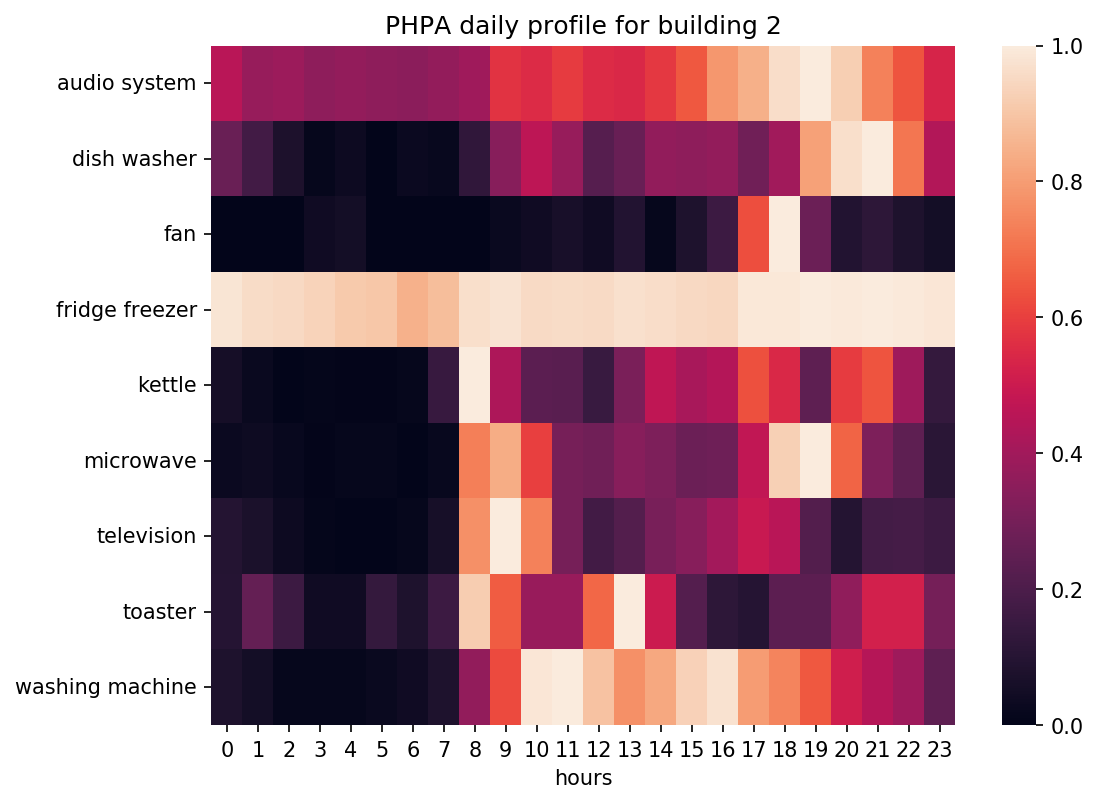
\includegraphics[width=1\linewidth]{../Figures/LPS/PHPA.png}
		\label{fig:ec_PHPA}
	\end{subfigure}%
	~ 
	\begin{subfigure}{.5\textwidth}
		% \centering
		\caption{"figure \protect\ref{arr:act_mat} as an image"}
		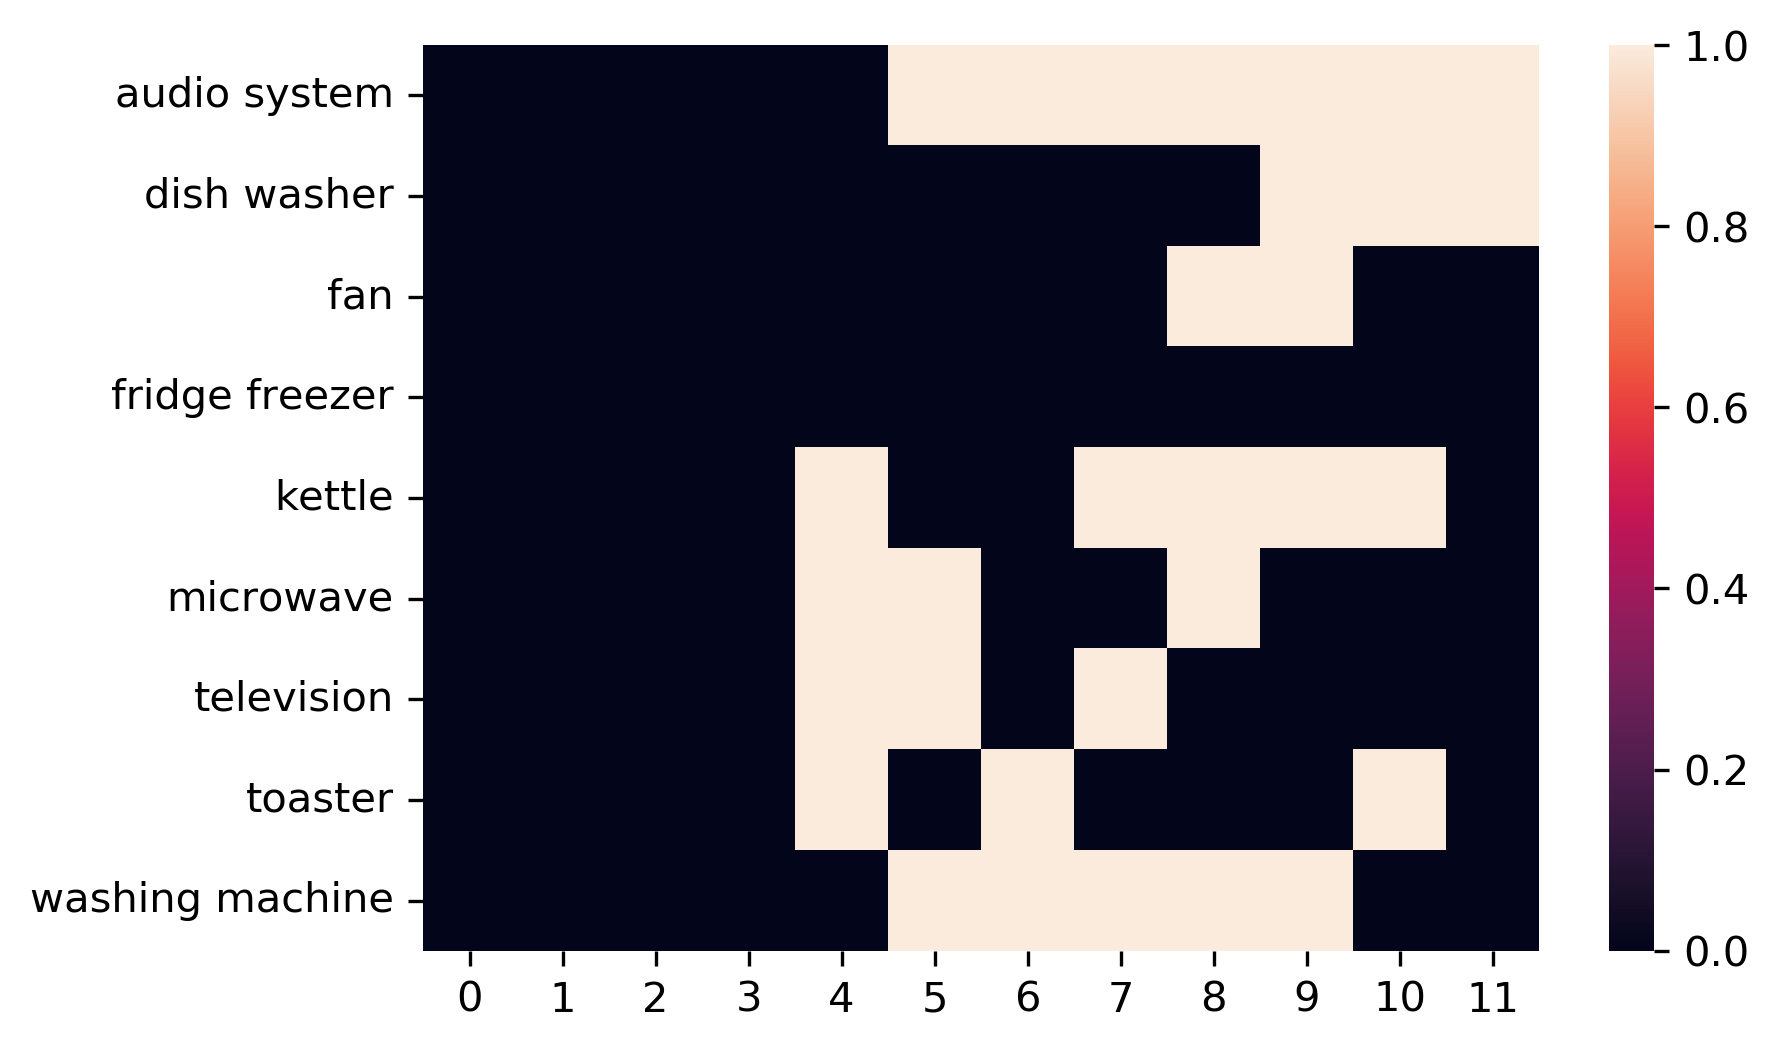
\includegraphics[width=1\linewidth]{../Figures/LPS/PHPA_EC.png}
		\label{fig:ec_PHPA_bw}
	\end{subfigure}%

	\caption{"Trasformation of source load profile to black and white"}
\end{figure}

\subsubsection{Step four}

Using the matrix \ref{arr:act_mat} we can write an algorithm that will use current activations 
and compare it to the matrix. For example, if we have the test sample for the fifth bucket, that is 
data from 8 to 10 o clock. 
What needs to be done is to use the fifth column and multiply the current activations.
Then anomaly is detected based on a rule: that at least two appliances must be activated, for the bucket to be labeled as normal,
or else the bucket is labeled as anomalous. In this case, we sum the elements of an array and check if it is larger or equal to 2. 

% \begin{figure}[H]
%     \centering
%     \begin{tikzpicture}
%         \coordinate (s) at (0,5);
%         \foreach \num in {0, 0, 0, 0, 0, 0, 0, 1, 1, 1, 1, 0}{
%         \node[minimum size=6mm, draw, rectangle] at (s) {\num};
%         \coordinate (s) at ($(s) + (1,0)$);
%         }
        
%         \node at (5.5,4) {X};
%         \coordinate (s) at (0,3);
%         \foreach \num in {1, 0, 0, 0, 0, 0, 0, 1, 0, 0, 1, 0}{
%         \node[minimum size=6mm, draw, rectangle] at (s) {\num};
%         \coordinate (s) at ($(s) + (1,0)$);
%         }
%         \node at (5.5,2){=};
%         \coordinate (s) at (0,1);
%         \foreach \num in {0, 0, 0, 0, 0, 0, 0, 1, 0, 0, 1, 0}{
%         \node[minimum size=6mm, draw, rectangle] at (s) {\num};
%         \coordinate (s) at ($(s) + (1,0)$);
%         }
%         \node at (5.5,0){SUM = 2 - > not an anomaly };
%     \end{tikzpicture}
%     \caption{The evaluation of new bucket compared to matrix. Example is for fifth bucket or fifth row from the matrix}
%     %\label{arr:microwave_acts_vec}
% \end{figure}

\begin{figure}[H]
    \centering
    \caption{"Process of evaluating an anomaly"}
    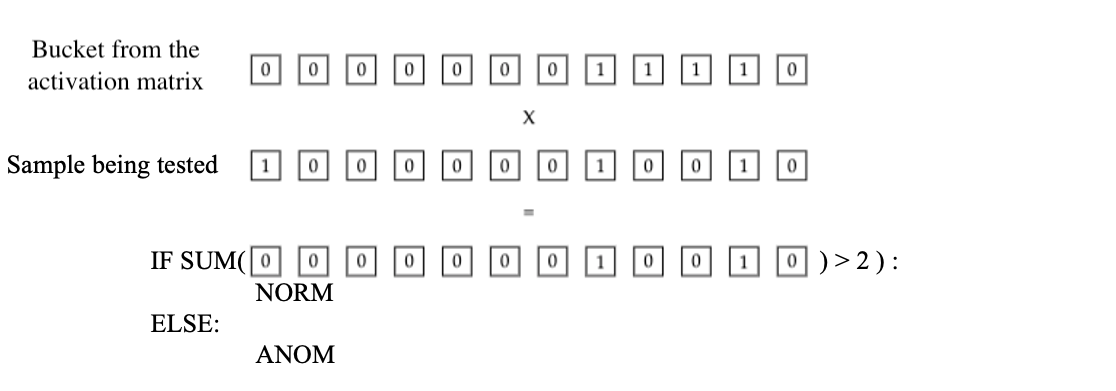
\includegraphics[width=1\linewidth]{../Figures/EC/EC_anom_dect.png}
    \label{fig:anom_detct}
    \caption{The evaluation of new bucket compared to matrix. Example is for fifth bucket or fifth row from the matrix}
    
\end{figure}

This process is done for all samples, where we count normal and anomalous samples for each bucket
The important thing to note here is that we are evaluating the samples from which the profile was built.

\begin{figure}[H]
    \centering
    \begin{tikzpicture}
        \coordinate (s) at (0,0);
        \foreach \num in {472, 469, 468, 466, 57, 153, 288, 187, 123, 84, 75, 281}{
        \node[minimum size=6mm, draw, rectangle] at (s) {\num};
        \coordinate (s) at ($(s) + (1,0)$);
        }
    \end{tikzpicture}
    \caption{Agregated anomalies for each bucket}
    \label{arr:agg_anom}
\end{figure}

\begin{figure}[H]
    \centering
    \begin{tikzpicture}
        \coordinate (s) at (0,0);
        \foreach \num in {0, 0, 0, 0, 409, 312, 181, 280, 342, 384, 394, 188}{
        \node[minimum size=6mm, draw, rectangle] at (s) {\num};
        \coordinate (s) at ($(s) + (1,0)$);
        }
    \end{tikzpicture}
    \caption{Agregated normal samples for each bucket}
    \label{arr:agg_norm}
\end{figure}

The next step is to combine these two arrays so that we calculate the percentage of anomalous samples 
for each bucket with an equation. 

\begin{equation}
    \frac{N_{anom}}{N_{anom}+N_{norm}}
    \label{eq:ratio}
\end{equation}

Where $N_{anom}$ is a number of anomalous samples and $N_{norm}$ is a number of normal samples.


We can alter the equation \ref{eq:ratio} so that it will measure
a number of normal samples out of all. 
The result is the equation \ref{eq:routine}
In other words, we are measuring the strength of a routine that 
user has in each bucket.

\begin{equation}
    R_{outine}= \frac{N_{norm}}{N_{anom}+N_{norm}}
    \label{eq:routine}
\end{equation}

Using the equation \ref{eq:routine} we can populate the array \ref{arr:anom_ratio}.

\begin{figure}[H]
    \centering
    \begin{tikzpicture}
        \coordinate (s) at (0,0);
        \foreach \num in {0.0, 0.0, 0.0, 0.0, 0.88, 0.7, 0.39, 0.6, 0.74, 0.82, 0.84, 0.4}{
        \node[minimum size=6mm, draw, rectangle] at (s) {\num};
        \coordinate (s) at ($(s) + (1,0)$);
        }
    \end{tikzpicture}
    \caption{Aggregated anomalies for each bucket}
    \label{arr:anom_ratio}
\end{figure}

In other words, the array \ref{arr:anom_ratio} tells us how persistent is the user's routine in each bucket or part of the day. 
The higher the metric the higher the routine. 
Since routine is detected based on the usage of appliances it cannot be picked up during the night.

It is possible to see that the routine is quite high during the morning and evening hours.
The anomaly detection algorithm will work best when the metric above is high.
A good trait of the elderly is that their routine is quite high even during the day,
which means that the anomaly detection will function better throughout the day.

One more thing to do is to ignore the parts of the day when the user has no routine, by using
the array \ref{arr:anom_ratio} and setting a threshold of 0.7. 

A threshold of 0.5 would mean that every other day could be a false positive anomaly. Setting the rate at 0.7 reduces that 
to every third day.
Here, compromises must be made, the lower the threshold the more accurate
the algorithm will be. This also means that it will be less sensitive. 
In our case, there is not much harm in false positives detections, since the caregiver can call
the elder to check if it is okay.  

\begin{figure}[H]
    \centering
    \begin{tikzpicture}
        \coordinate (s) at (0,0);
        \foreach \num in {0, 0, 0, 0, 1, 1, 0, 0, 1, 1, 1, 0}{
        %\foreach \num in {1.0, 1.0, 1.0, 1.0, 0.12, 0.3, 0.61, 0.4, 0.26, 0.18, 0.16, 0.6}{
        \node[minimum size=6mm, draw, rectangle] at (s) {\num};
        \coordinate (s) at ($(s) + (1,0)$);
        }
    \end{tikzpicture}
    \caption{Using above-mentioned threshold a new mask is made, to check only buckets with high routine}
    \label{arr:anom_ratio_mask}
\end{figure}

\subsubsection{Step five}

The last step is to repeat steps 4 and 5 with data, that is not included in the built profile.


\subsection{Datasets and evaluation} \label{ssec:ds_eval}

The data was split into train and test sets, where 80 \% of the data was for training and 20 \% percent of the data was used for testing.
The data was split based on the number of samples, so in some cases where there is a lot of missing data, the time window of test data might be longer, although it contains only 20 \% of the samples.

\subsubsection{REFIT}
The REFIT \cite{REFIT} dataset included data for more than 15 buildings, as can be seen on the figure below.
The dataset in general is of the highest quality since it is the longest with the least missing data.
This means this dataset should give the most relevant results.
\begin{figure}[H]
	\centering
	\caption{"Timeline for REFIT "}
	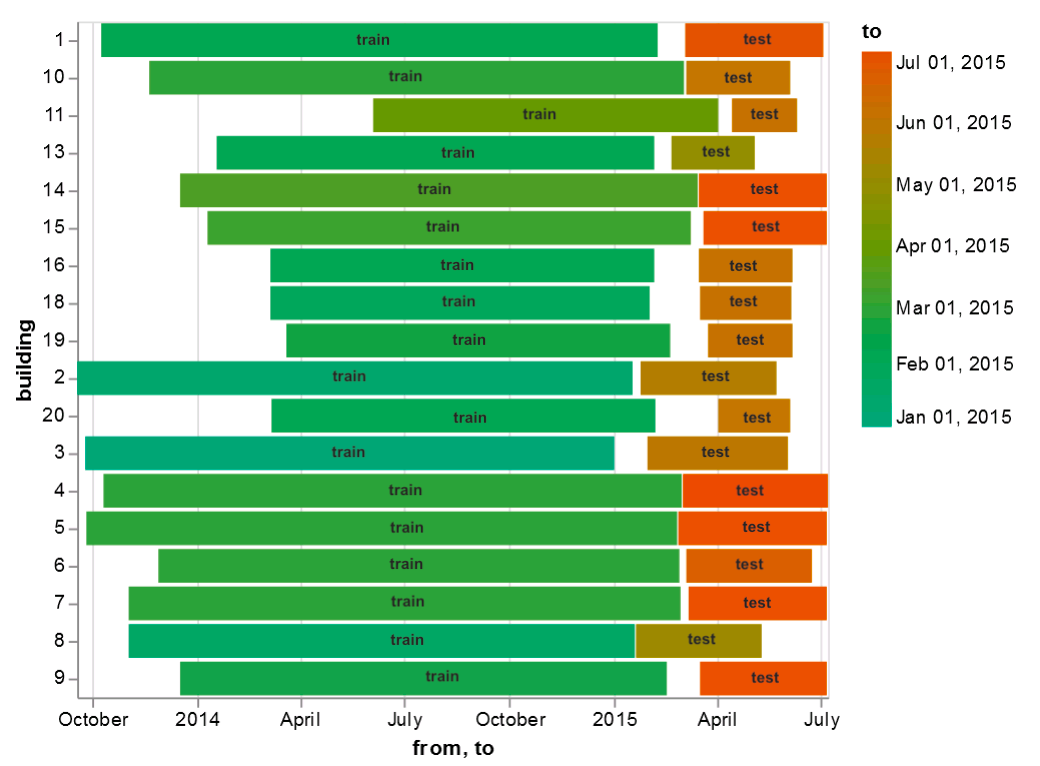
\includegraphics[width=1\textwidth]{Figures/EC/refit_timeline.png}
	\label{fig:refit_timeline}
\end{figure}

\subsubsection{UK-DALE} 

All through the UK-DALE \cite{UKDALE} dataset is of similar size, the most of the data is from building 1.
In general, it includes 5 years of data, but only for some appliances, where many appliances are rarely used.
When taking all of this into account, there were too many issues with building 1, and it was simply ignored.
Another issue that can be seen on \ref{fig:ukdale_timeline} is that there is not enough data for 
building 3. The test includes only a week of data, which is not enough for representative results, therefore it was ignored.
The rest of the buildings seem healthy.

\begin{figure}[H]
	\centering
	\caption{"Timeline for UK-DALE "}
	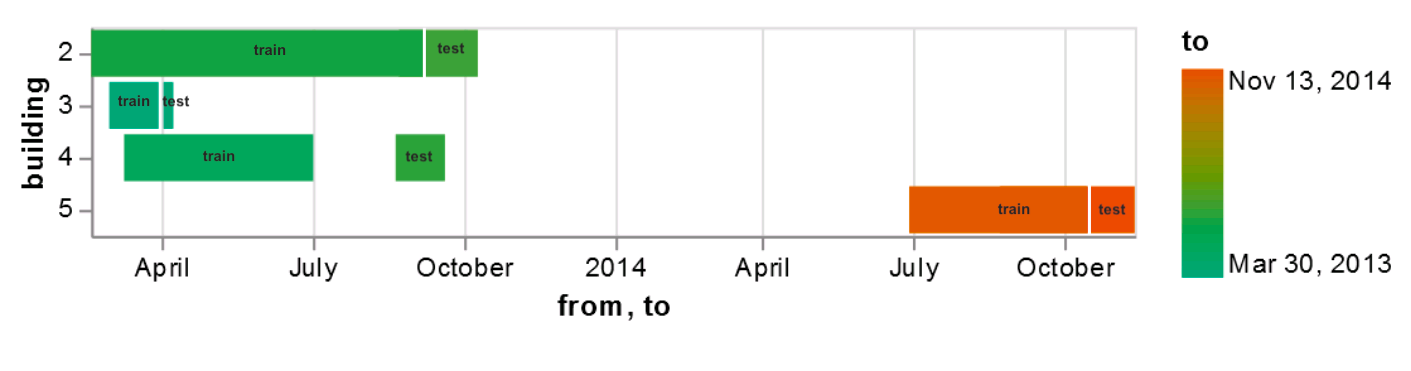
\includegraphics[width=1\textwidth]{Figures/EC/ukdale_timeline.png}
	\label{fig:ukdale_timeline}
\end{figure}

\subsubsection{ECO}
ECO \cite{ECO} dataset has a length of data, similar to UK-DALE. 
The only issue is building 1, where there is a lot of missing data.
This is a good example of how data is split, it is split based on several samples,
meaning that there is 80 \% in the train bar, due to missing data the second bar is longer. 

\begin{figure}[H]
	\centering
	\caption{"Timeline for ECO"}
	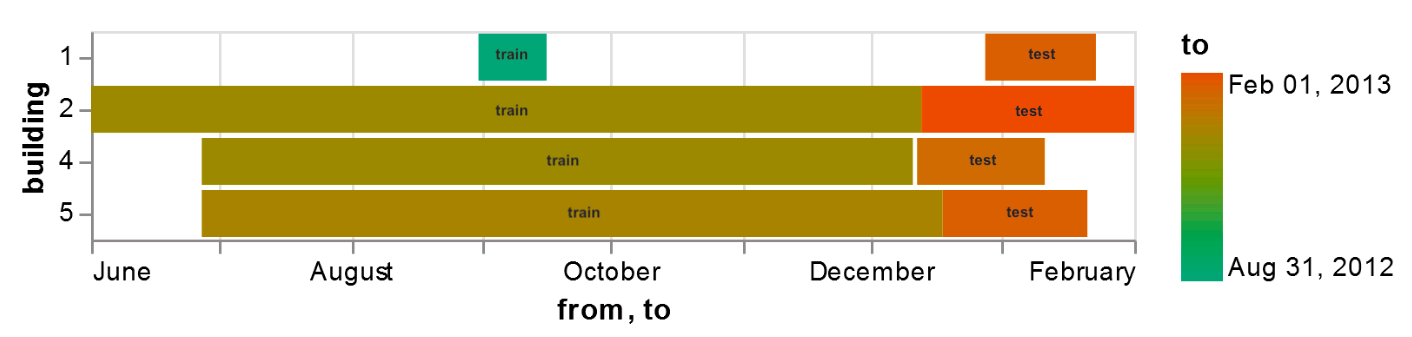
\includegraphics[width=1\textwidth]{Figures/EC/eco_timeline.png}
	\label{fig:eco_timeline}
\end{figure}


\subsection{The metric - routine rate}

Due to the lack of ground truth data of actual accidents, it is hard to determine the 
exact accuracy of this algorithm. Every anomaly detected is not necessarily an 
actual accident, it could be that the user decided to lie in bed a bit longer, or decided to go to bed early in the evening.
One metric that we can use to determine how well the algorithm functions is the routine rate metric \ref{arr:anom_ratio}.
The reason behind that is, that if the routine rate is high it means that it will be easier to detect the actual anomaly.

\begin{itemize}
	\item routine rate of 0 would mean that for that bucket household has no routine at all.
    \item routine rate of 0.5 would mean that the routine is being "practiced" every second day
    \item routine rate of 0.8 would mean that routine is broken on average every 5 day
    \item routine rate of 1 would mean that this household has a routine that is never broken. 
\end{itemize}

When a true anomaly occurs such as a fall, the dweller, all through he had the same strong routine for the past year (the routine rate would be close to 1), would not be able to practice the routine, and the algorithm will be quite sure that this is an actual anomaly.
Therefore, the lower the routine rate the less sure we are that an actual anomaly such as a fall occurred.
This is a good alternative measurement, that tells us how well this algorithm will perform. 
Since sometimes it is easier to read when results are presented with percentages, we will sometimes use this way of writing it.
 
\section{Results} 

Results were obtained for 3 datasets. 
REDD and iAWE datasets were not used, since the dataset was too short. 
They contained less than a month of data. 

\subsection{The routine rate over a period of time}

In the following sections, we will present how the metric changes over given periods of time.
This will enable us to see that there are patterns that this metric helps reveal. 
Since we have more than a year of training data, this will enable us to see how the metric changes over years time.
This enables us to see how routine changes over the year. 
We cannot use testing data in this case, since there is not enough of it.

\subsubsection{The routine rate through the week} \label{sssec:ratio_week}

As the behavior of the dwellers' changes, so does the accuracy of the algorithm. 
One observation that was made, was that the routine was higher during the week than during the weekends,
as can be seen in the figure \ref{fig:ec_week} below. 
The figures also show that for different houses, the change in routine also differs.
The only exception is building 5, which shows that the observation does not hold for all houses. 

\begin{figure}[H]
	\begin{subfigure}{.5\textwidth}
		% \centering
		\caption{"Building 2"}
		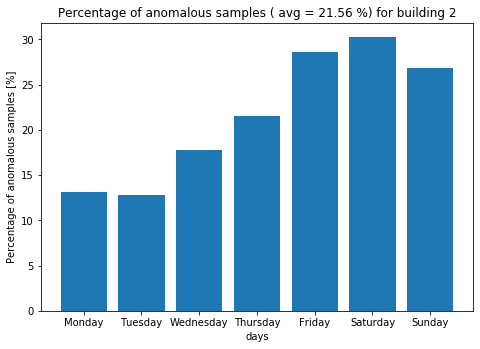
\includegraphics[width=1\linewidth]{../Figures/EC/b2week.png}
		\label{fig:ec_b2week}
	\end{subfigure}%
	~ 
	\begin{subfigure}{.5\textwidth}
		% \centering
		\caption{"Building 19"}
		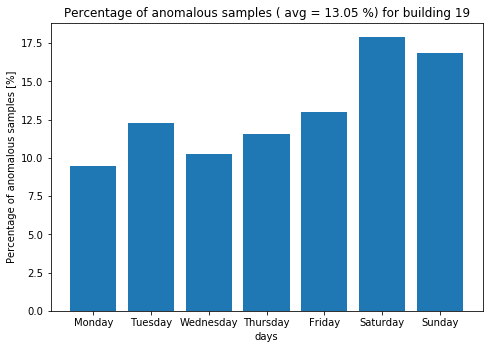
\includegraphics[width=1\linewidth]{../Figures/EC/b19week.png}
		\label{fig:ec_b5week}
	\end{subfigure}%
    \bigskip

    \begin{subfigure}{.5\textwidth}
		% \centering
		\caption{"Building 18"}
		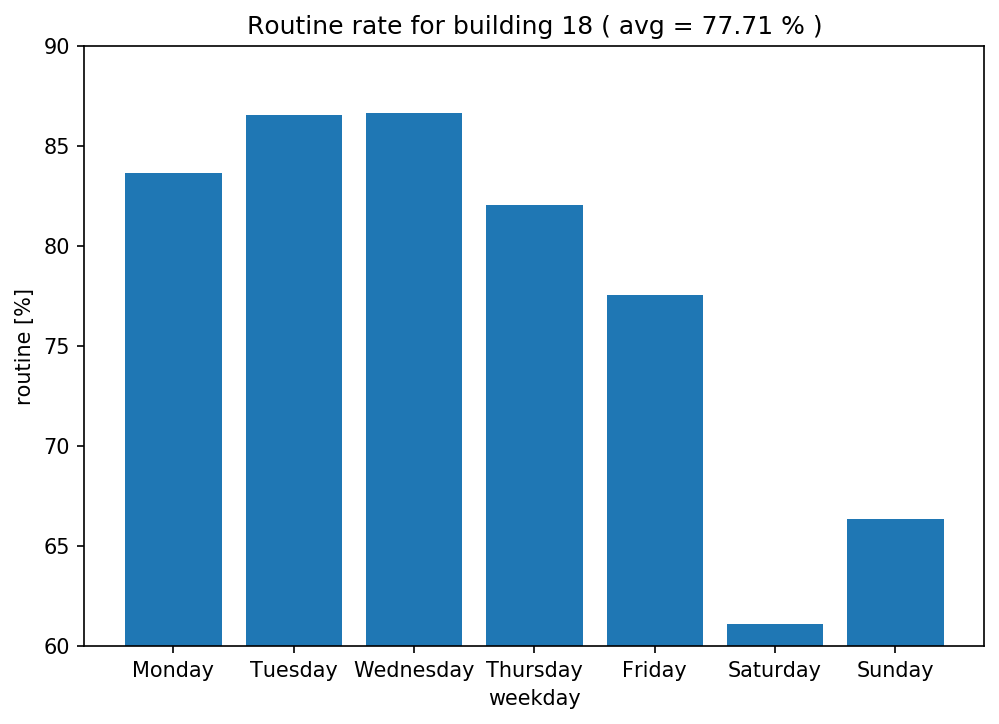
\includegraphics[width=1\linewidth]{../Figures/EC/b18week.png}
		\label{fig:ec_b18week}
	\end{subfigure}%
    ~ 
    \begin{subfigure}{.5\textwidth}
		% \centering
		\caption{"Building 5"}
		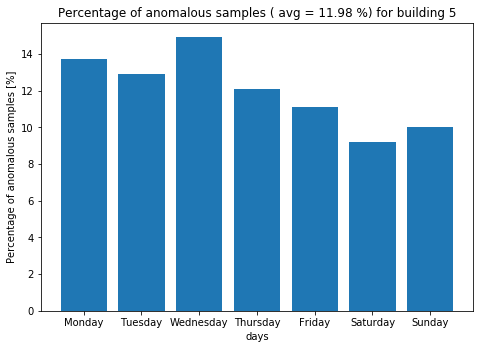
\includegraphics[width=1\linewidth]{../Figures/EC/b5weekd.png}
		\label{fig:ec_b5week}
	\end{subfigure}%
	\label{fig:ec_week}
	\caption{"Routine rate through the week (train data)"}
\end{figure}


Since we are dealing with the elderly, they have a higher routine, and it does not change that much during the weekends. 
Usually, assisted living systems are put in place since elders are alone in the dwelling.
Taking all of this into account, we could assume that the routine of the elderly is the same trough the week and simply ignore the weekends. 
This should yield more relevant results. 

\subsection{Routine rate through a year}

The rate at which the routine is being practiced also changes over a year. 
While on average the routine rate is higher during the winter, spring and summer, it is lower during the summer due to vacation. 
This can be seen in the figure \ref{fig:ec_year} below. 
It is possible to observe dips in routine. 
In some cases, these dips occur in summer and others in springtime. 
Without metadata, we cannot know for sure, what was the event behind these dips. 
There is a high chance most of them are vacations or other events where one or more dwellers are away from home for extended periods of time. 

\begin{figure}[H]
	\begin{subfigure}{.5\textwidth}
		% \centering
		\caption{"Building 2"}
		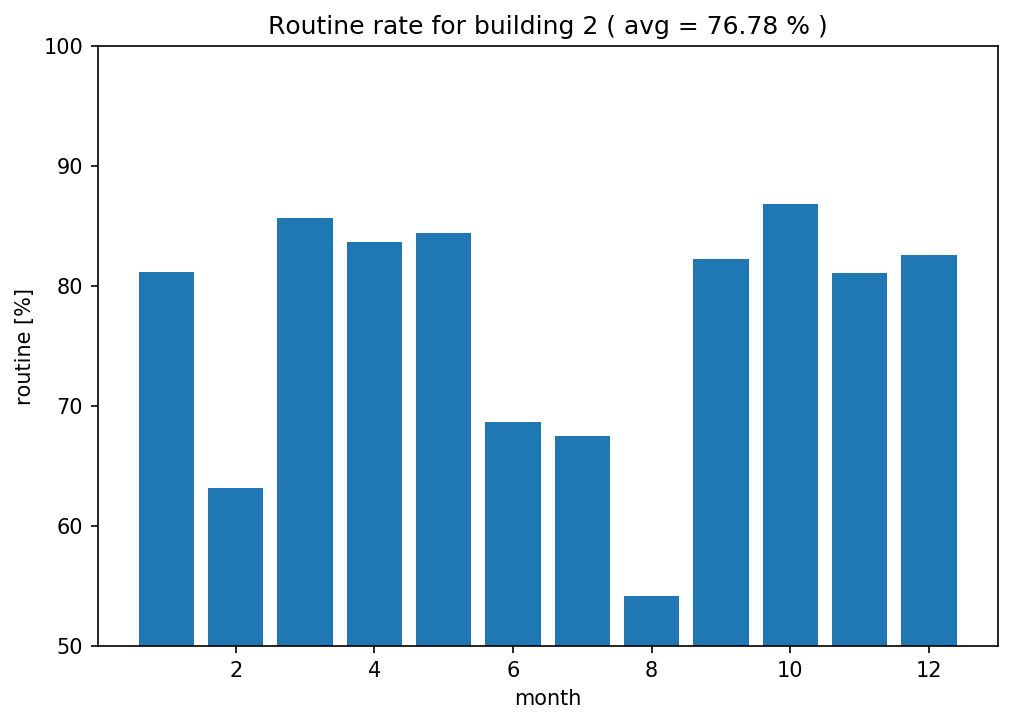
\includegraphics[width=1\linewidth]{../Figures/EC/b2year.png}
		\label{fig:ec_b2year}
	\end{subfigure}%
	~ 
	\begin{subfigure}{.5\textwidth}
		% \centering
		\caption{"Building 19"}
		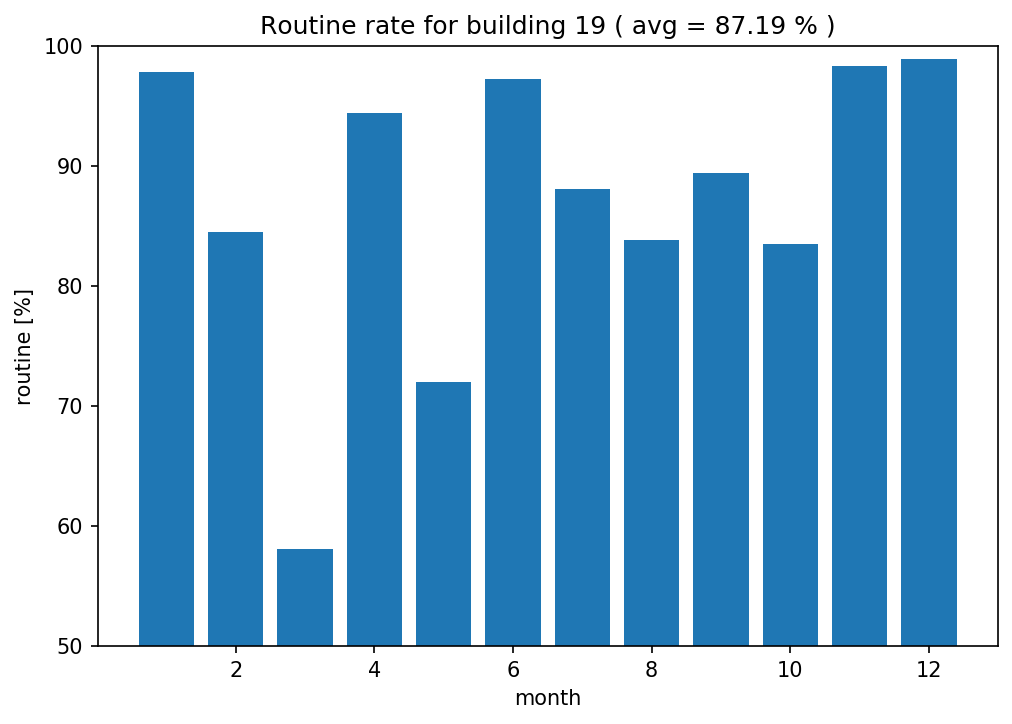
\includegraphics[width=1\linewidth]{../Figures/EC/b19year.png}
		\label{fig:ec_b5year}
	\end{subfigure}%
    \bigskip

    \begin{subfigure}{.5\textwidth}
		% \centering
		\caption{"Building 18"}
		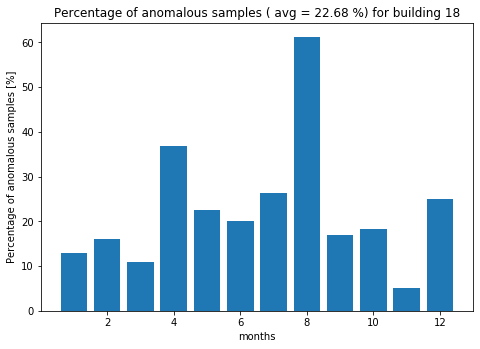
\includegraphics[width=1\linewidth]{../Figures/EC/b18year.png}
		\label{fig:ec_b18year}
	\end{subfigure}%
    ~ 
    \begin{subfigure}{.5\textwidth}
		% \centering
		\caption{"Building 5"}
		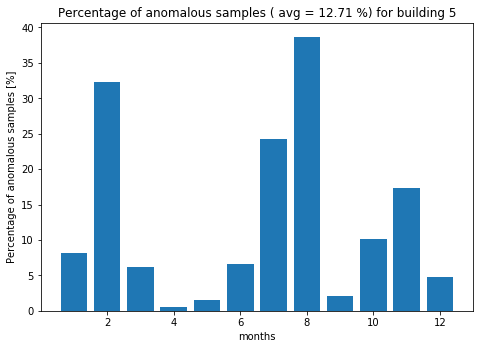
\includegraphics[width=1\linewidth]{../Figures/EC/b5year.png}
		\label{fig:ec_b5year}
	\end{subfigure}%
	\label{fig:ec_year}
	\caption{"Routine through the year (train data)"}
\end{figure}

\subsection{Effectiveness of anomaly detection through the day}

The following subsection will show how the effectiveness of anomaly detection changes throughout the day.

One thing to keep in mind is that this algorithm will be able to detect anomalies only when
the routine will be high, and more than two appliances will be used in given buckets.

Figure \ref{fig:ignored_buckets_22} shows which buckets were most commonly used for the detection of an anomaly.
The graph includes averaged values from all buildings and datasets. 
In other words, the graph presents how strong is average routine through the day.

This means that the higher the routine, the higher the chance that this bucket will be used for anomaly detection.
During the night, it is possible to see that the average routine rate is quite high.
This can be seen in figure \ref{fig:ignored_buckets_22}
this is because most users are routinely sleeping during that period.
But as we can see in figure \ref{fig:ignored_buckets_22},
the high routine rate does not necessarily mean the buckets are useful.

\begin{figure}[H]
	\centering
	\caption{"Effectivnes of anomaly detection through the day"}
	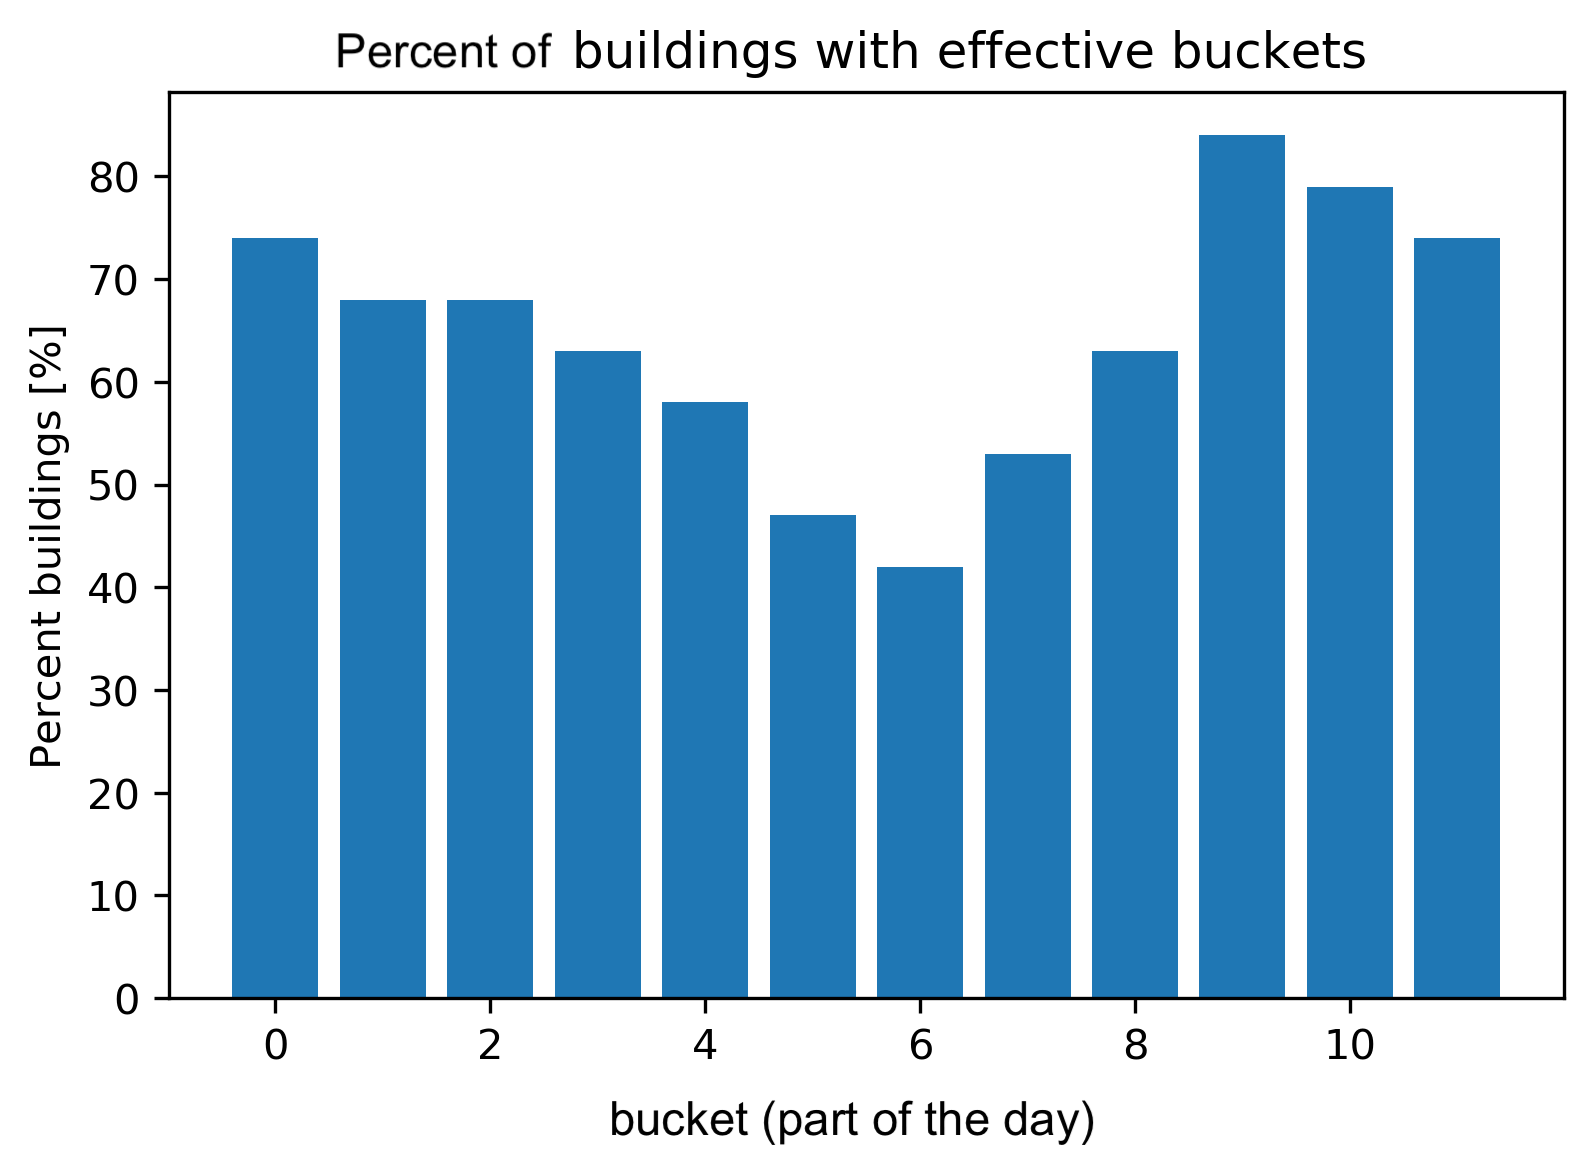
\includegraphics[width=.8\textwidth]{Figures/EC/ignored_buckets_dist.png}
	\label{fig:ignored_buckets_22}
\end{figure}

To find the usable buckets, an additional filter must be applied.
The rule is that at least two appliances must be commonly used in that bucket. 
After applying this rule the following figure emerges \ref{fig:ignored_buckets_act}

\begin{figure}[H]
	\centering
	\caption{"Actual effectiveness of anomaly detection through the day"}
	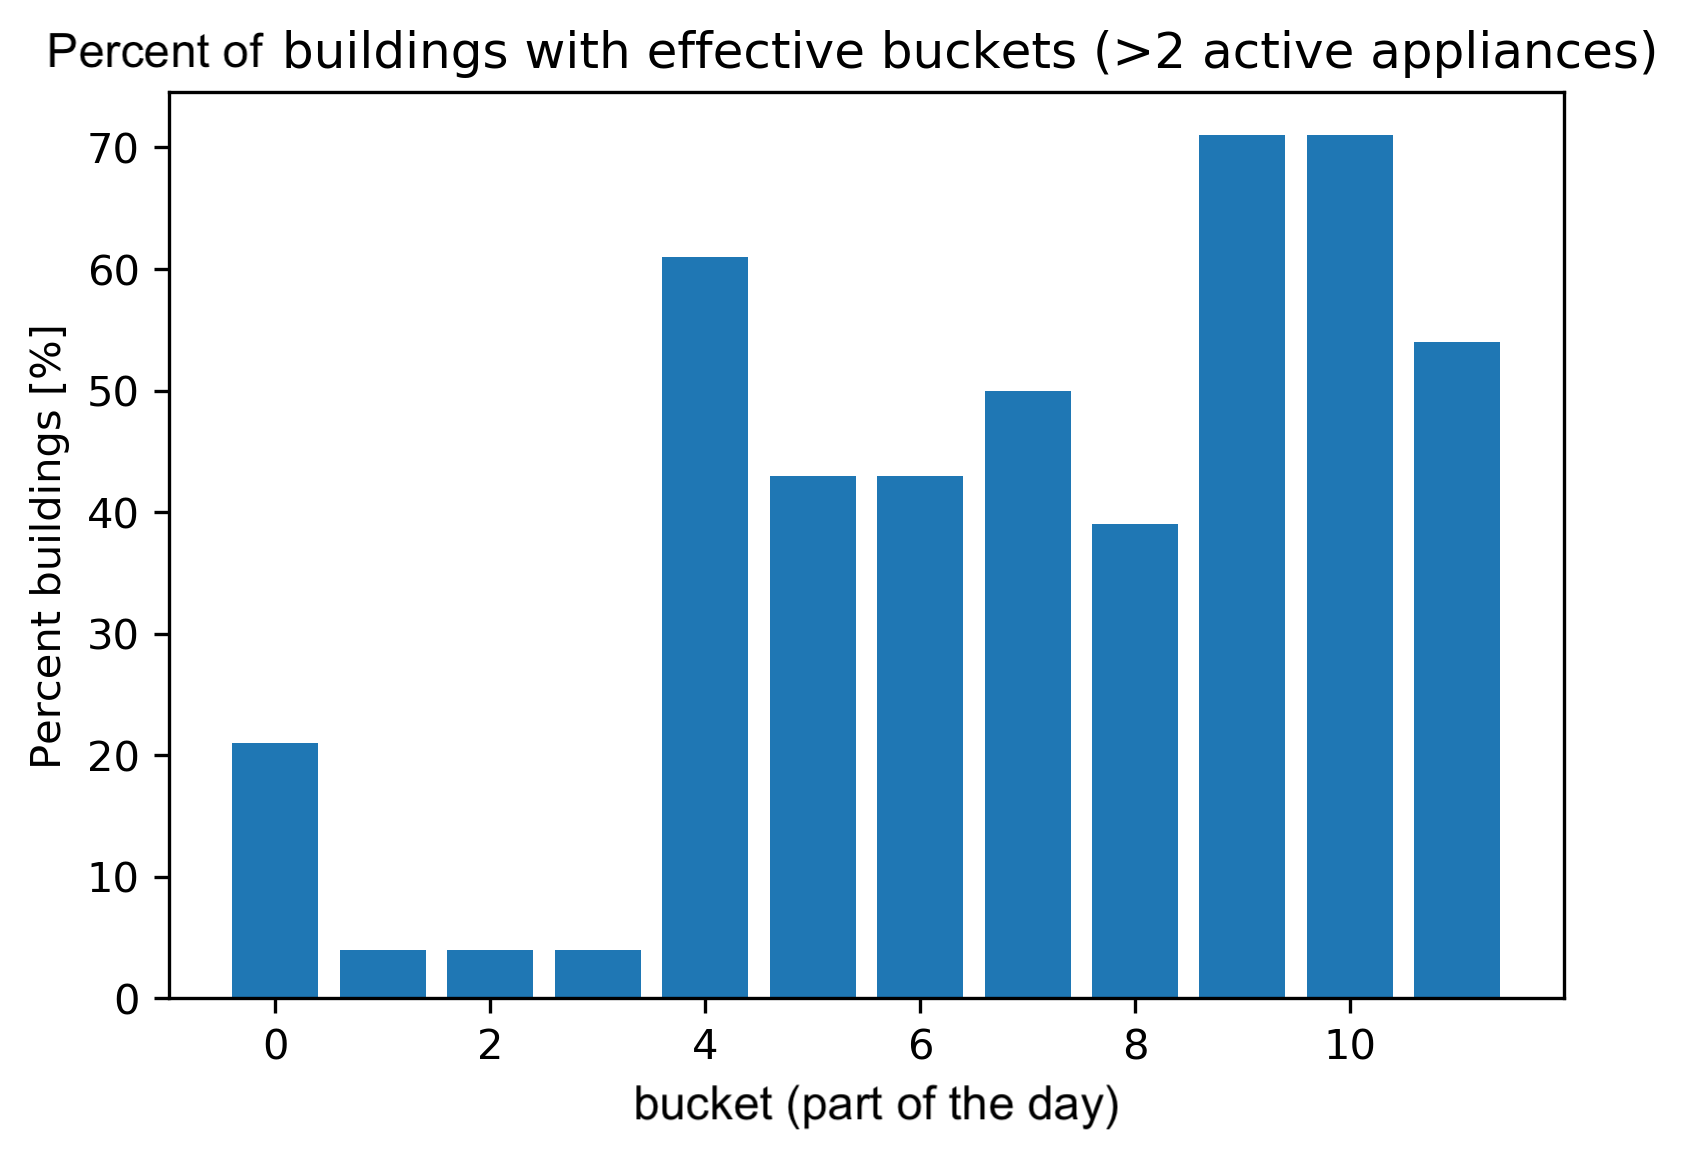
\includegraphics[width=.8\textwidth]{Figures/EC/all_ignored_buckets_dist_incl_act.png}
	\label{fig:ignored_buckets_act}
\end{figure}

The figure \ref{fig:ignored_buckets_act} shows that there are two peaks.
One in the morning and the other, a wider one in the evening.

This means that on an average home the algorithm would perform best in the morning and evening.
This is because the average person is at school or work during noon. 
This can be confirmed on figure \ref{fig:ignored_buckets_act}.
The elderly, are usually at home at noon, which could extend the effective detection window.


\subsubsection{The anomaly detection during the night}

We have seen that anomalies can be detected throughout the day,
but are hard to detect through the night, since appliances are off.

This is because, in our current state, an anomaly occurs when something that should operate, does not.
When the user is sleeping, an anomaly occurs when something that shouldn't operate, does. 
To implement this additional rule, we would have to build two models.
One would be online during the day, and the other when the user is sleeping.

To obtain the information about users sleep schedule, we could either have a schedule obtained from the user or we could extract it based on the usage pattern of appliances.
You can easily detect when most of the appliances are inactive, and build a sleep profile based on this information.

Using the sleep schedule, we cloud easily switch between the two operating modes. 
This new implementation would further extend the windows within which we can detect the anomalies and thus further improves users' safety.

The main issue here is not the detection itself but efficiently detecting
when the user is sleeping. 

The examples above were a demonstration and a look into data and metrics. 
The examples shown were trained and evaluated on the same data. 
To show true performance, we will use test data to determine the actual performance. 


\subsection{Per-building results}
\subsubsection{REFIT}

Results show, that the method is on average 76.4 \% efficient for REFIT.  
In figure \ref{fig:refit_res} it is possible to see that house 6 yields much better results and house 13 much worse than the rest. 
This could be due to various dataset errors that occurred during sampling.

\begin{figure}[H]
	\centering
	\caption{"Results for REFIT "}
	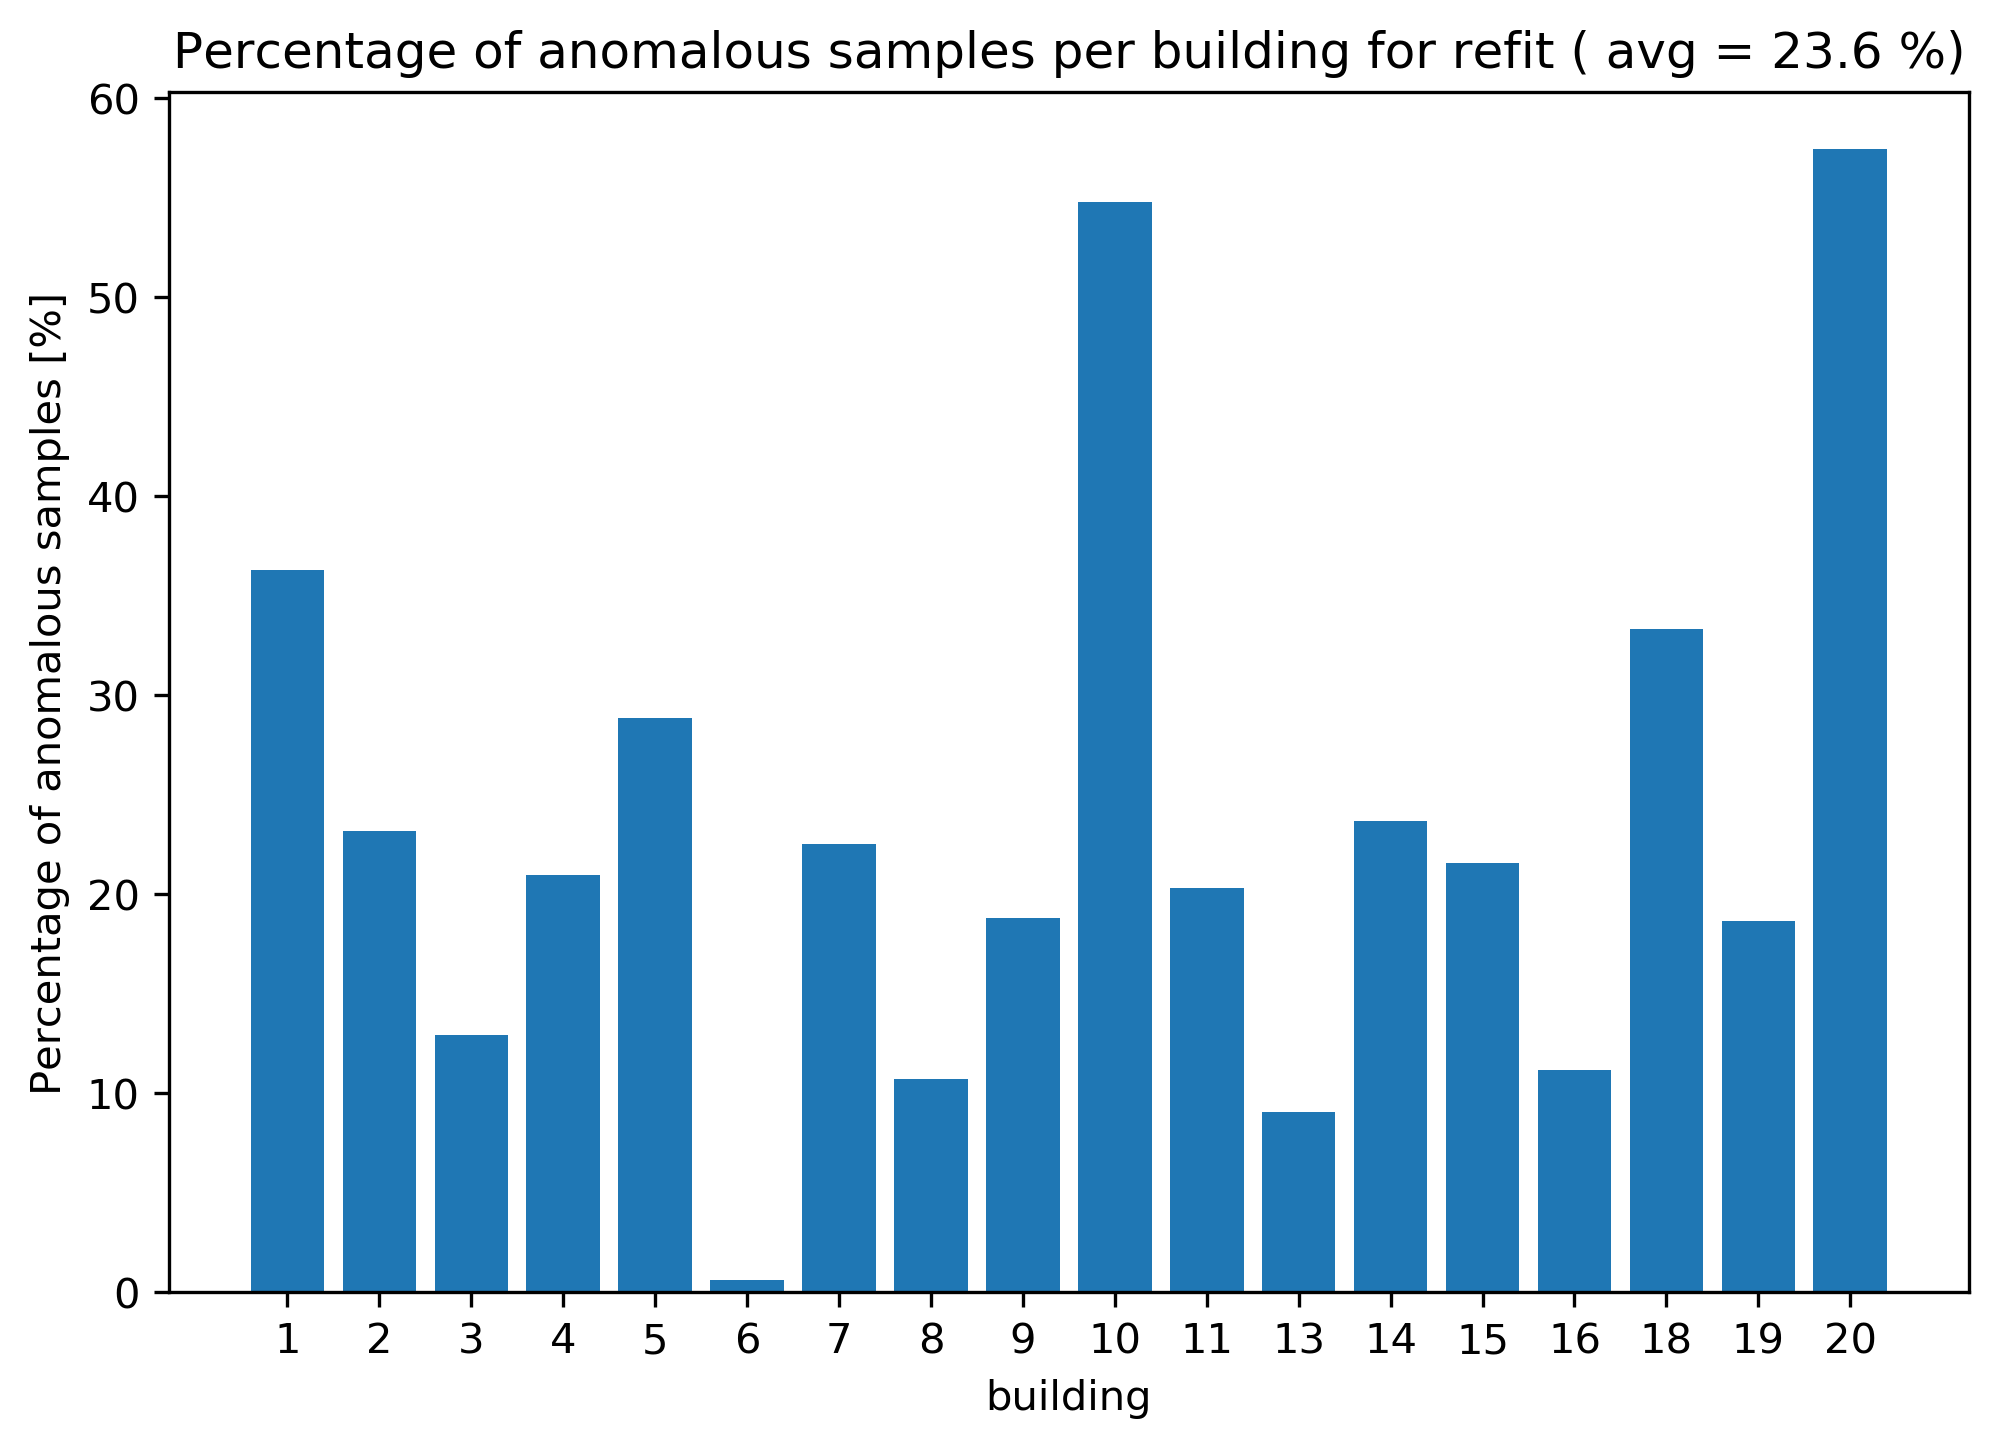
\includegraphics[width=.8\textwidth]{Figures/EC/refit_res.png}
	\label{fig:refit_res}
\end{figure}

For more relevant results we can ignore the outliers by removing one maximum and minimum value, such as can be seen in figure \ref{fig:refit_res2}
This yields a result of 77.08 \%.
If we were to repeat this process the result would be 79.77 \%.
Since all outliers are removed, the result converges towards 79 \%, which is the relevant value. 

\begin{figure}[H]
	\centering
	\caption{"Results for REFIT with removed outliers "}
	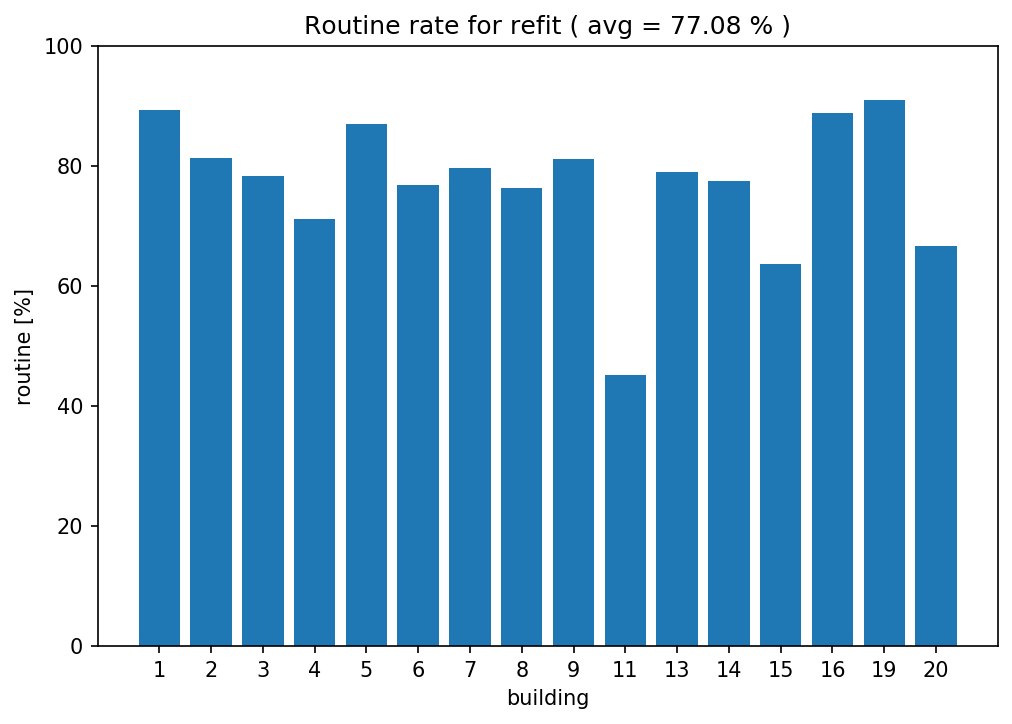
\includegraphics[width=.8\textwidth]{Figures/EC/refit_res2.png}
	\label{fig:refit_res2}
\end{figure}


As mentioned in the sub-sub section \ref{sssec:ratio_week}, the average routine is different during the week and weekends.
The assumption was that the routine of elderly people does not change significantly over the week, therefore results should be more relevant if we ignore the weekends.
The results on figure \ref{fig:refit_res_nw_1"} show that result improved to 77.08 \%.

\begin{figure}[H]
	\centering
	\caption{"Results for REFIT weekday only"}
	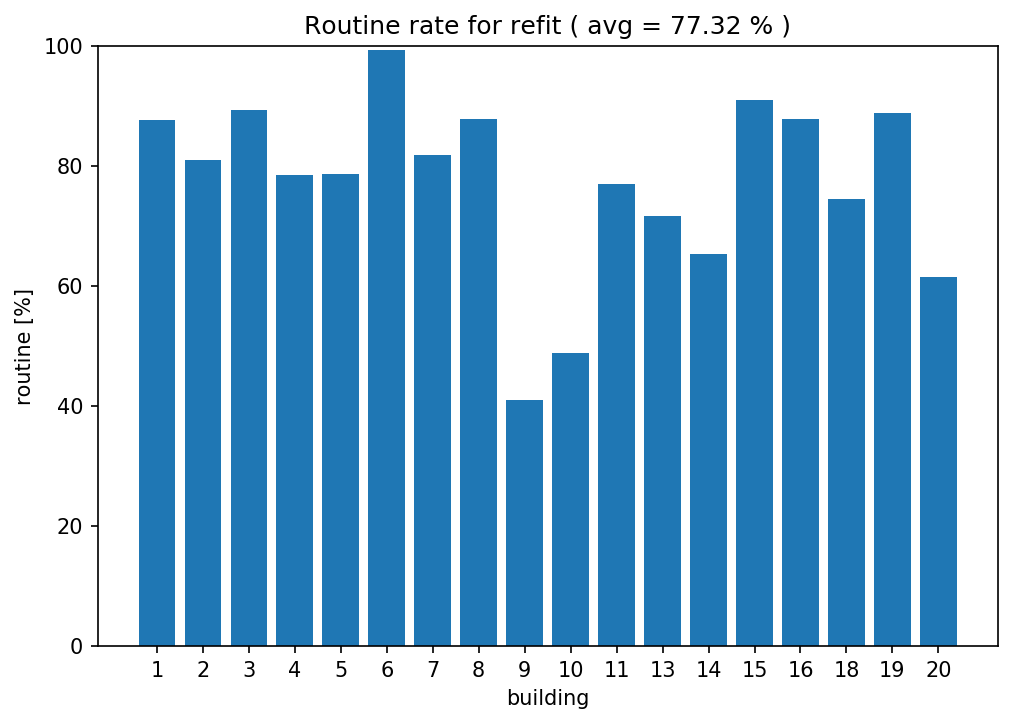
\includegraphics[width=.8\textwidth]{Figures/EC/refit_res_nw_1.png}
	\label{fig:refit_res_nw_1"}
\end{figure}

By ignoring the minimal and maximal outliers the results increase to 78.21 \%.
By repeating the process one more time the result increases to 80.20 \%, since all outliers were removed, the result converges towards this value. 

By removing the weekend data, the results improved by 1.2 \%. 

\begin{figure}[H]
	\centering
	\caption{"Results for REFIT weekday only and removed outliers"}
	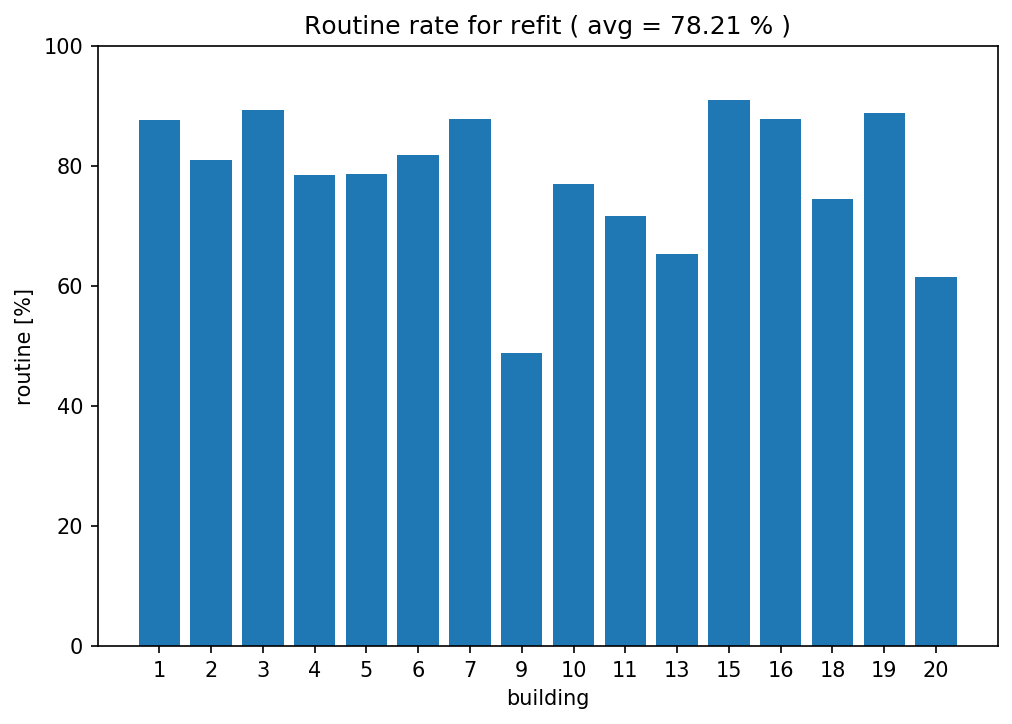
\includegraphics[width=.8\textwidth]{Figures/EC/refit_res_nw_2.png}
	\label{fig:refit_res_nw_2"}
\end{figure}

\subsubsection{UK-DALE}

As mentioned in subsection \ref{ssec:ds_eval}, the UK-DALE is not as big and cleaned as the previous dataset, so the results could be less relevant.
The results on figure \ref{fig:ukdale_res}, show that the average result is 74.48 \%. 
Due to the low number of buildings, it is not possible to detect and ignore outliers.

\begin{figure}[H]
	\centering
	\caption{"Results for UK-DALE"}
	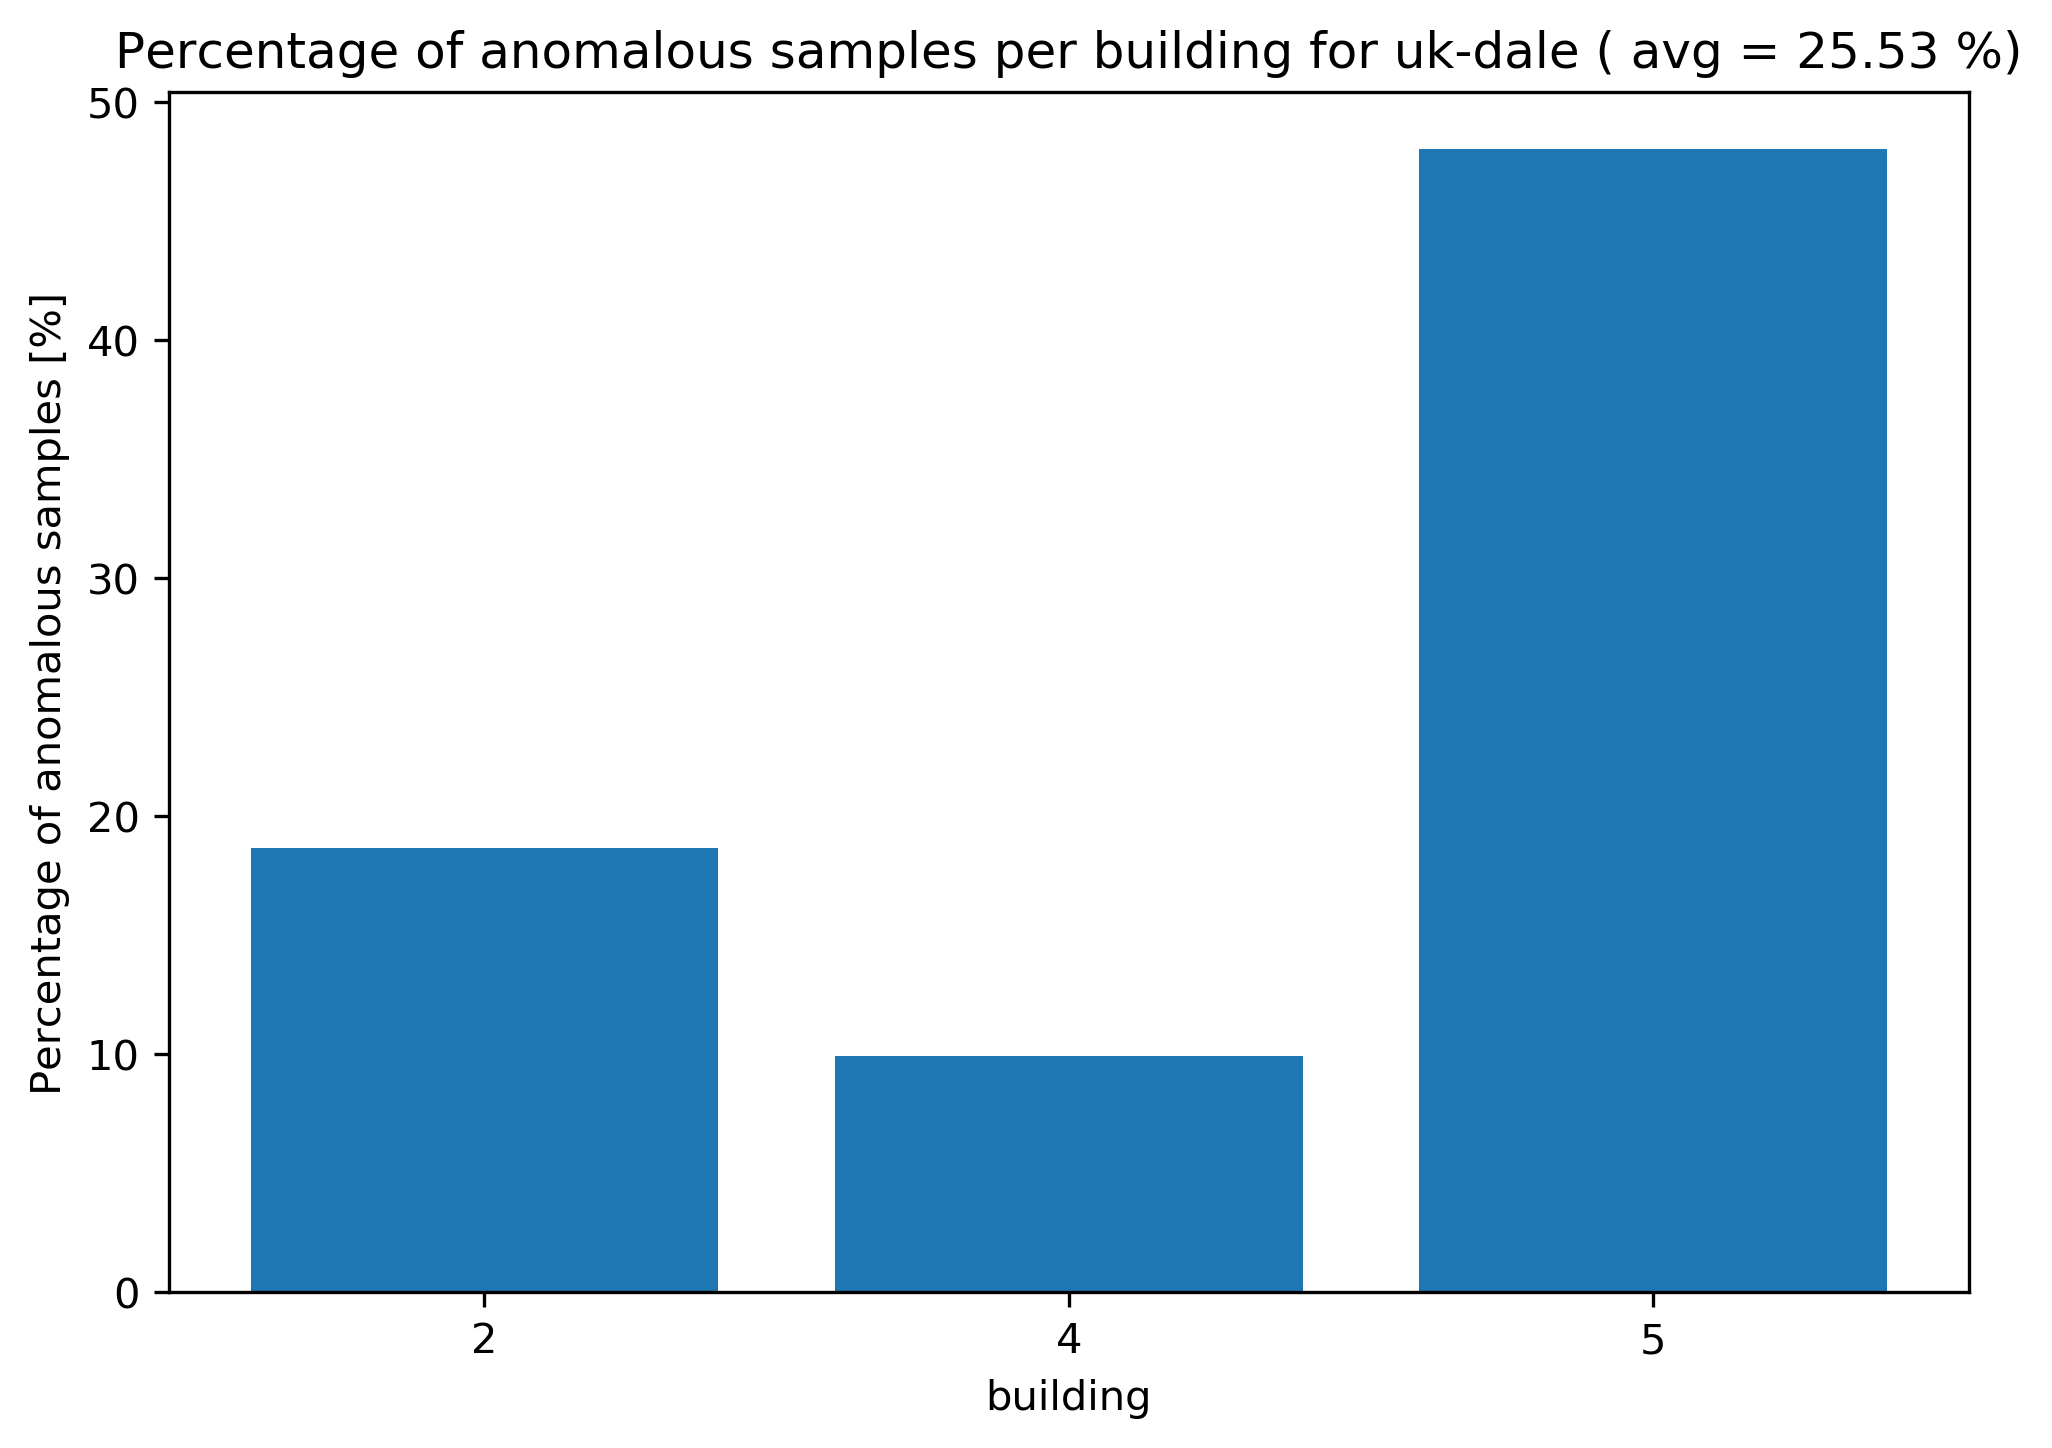
\includegraphics[width=.7\textwidth]{Figures/EC/ukdale_res.png}
	\label{fig:ukdale_res}
\end{figure}

The same as for REFIT, the weekend data can be ignored,
In this case, this does not improve the result. 

\begin{figure}[H]
	\centering
	\caption{"Results for UK-DALE omitinng weekends "}
	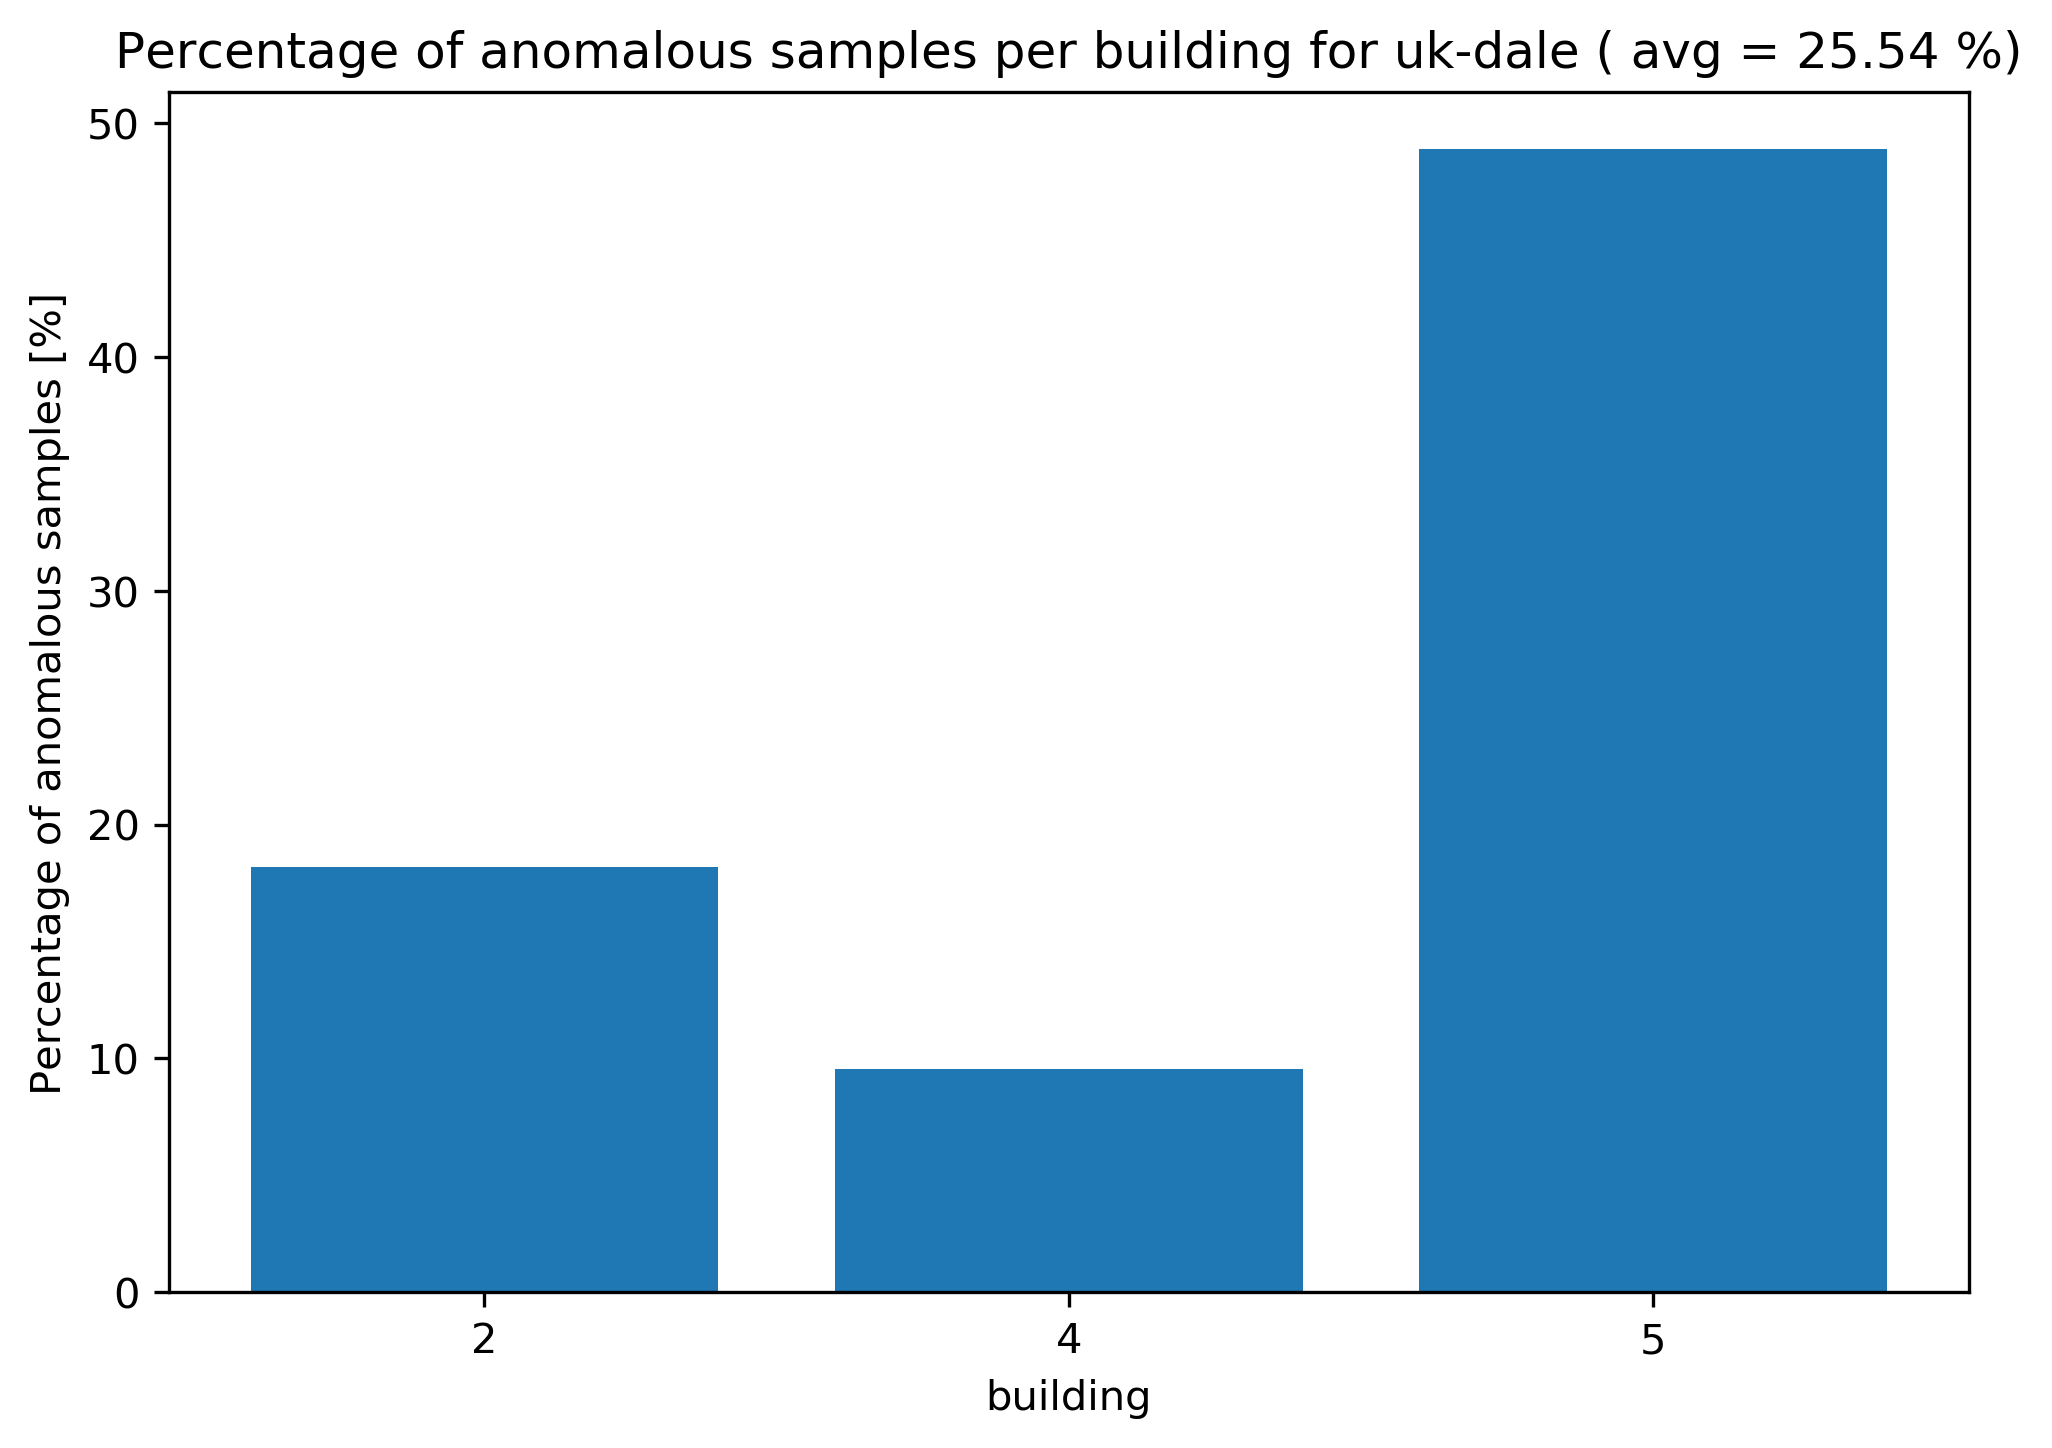
\includegraphics[width=.7\textwidth]{Figures/EC/ukdale_nw_res.png}
	\label{fig:ukdale_res_nw}
\end{figure}

\subsubsection{ECO}

ECO is of a similar quality as UK-DALE regarding the number of buildings and the length of data.
This can be seen in \ref{ssec:ds_eval}
The results \ref{fig:eco_res}, show that this dataset performed the best, with results of 84.09 \%.

\begin{figure}[H]
	\centering
	\caption{"Results for ECO "}
	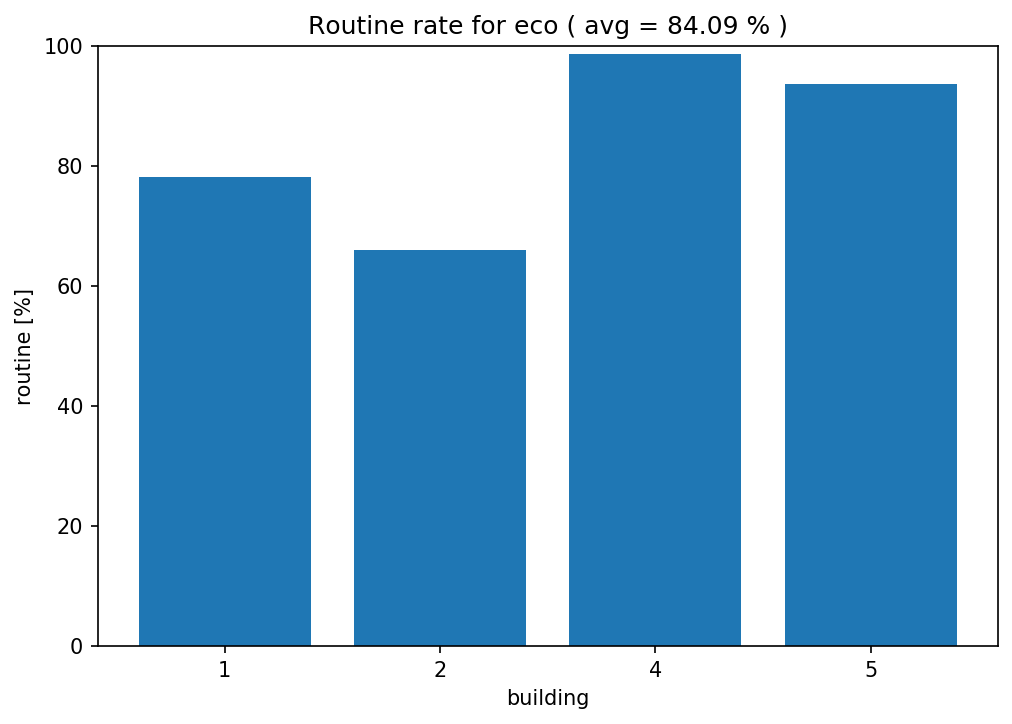
\includegraphics[width=.7\textwidth]{Figures/EC/eco_res_nw_1.png}
	\label{fig:eco_res}
\end{figure}

The same as before we can omit weekend data, which can be seen on \ref{fig:eco_res_nw}. This brings the result down to 83.80 \%. 

\begin{figure}[H]
	\centering
	\caption{"Results for ECO omiting weekends "}
	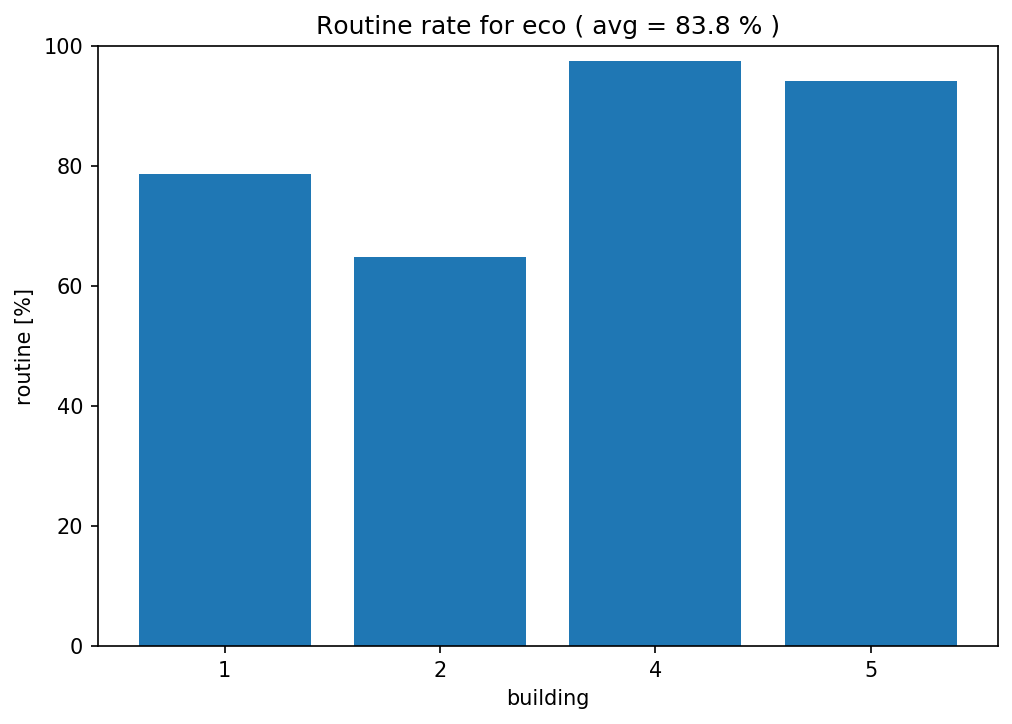
\includegraphics[width=.7\textwidth]{Figures/EC/eco_res.png}
	\label{fig:eco_res_nw}
\end{figure}

\subsection{Combined results}

After combining results from all 25 buildings, the table \ref{tab:ec_res} can be populated.
The most relevant results can be seen in the last row.
\begin{table}[H]
    \centering
    \caption{Combined percentage of anomolous samples [\%]}
    \begin{tabular}{|l|ll|ll|}
    \hline
    N = 25 &
      \multicolumn{2}{l|}{\begin{tabular}[c]{@{}l@{}}Including \\ weekend data\end{tabular}} &
      \multicolumn{2}{l|}{\begin{tabular}[c]{@{}l@{}}Excluting \\ weekend data\end{tabular}} \\ \hline
    \begin{tabular}[c]{@{}l@{}}Removed \\ min/max\\ outliers\end{tabular} &
      \multicolumn{1}{l|}{train } &
      test &
      \multicolumn{1}{l|}{train} &
      test \\ \hline
    0 & \multicolumn{1}{l|}{84.73} & 77.35 & \multicolumn{1}{l|}{86.20} & 78.07 \\ \hline
    1 & \multicolumn{1}{l|}{84.63} & 77.91 & \multicolumn{1}{l|}{86.16} & 78.75 \\ \hline
    2 & \multicolumn{1}{l|}{86.53} & 78.53 & \multicolumn{1}{l|}{86.13} & 79.23 \\ \hline
    \end{tabular}
    \label{tab:ec_res}
\end{table}

Results show that the algorithm is 78 \% efficient at detecting true anomalies. 
On average, the algorithm would label 22 \% of samples as false positives, 
in other words, every fifth sample could be a false positive. 

The nature of this system is that there is more harm done if we do not detect an anomaly than if we detect a few false positives. 
Therefore, in short, we can claim that the performance of this algorithm is adequate to be used in the real world. 

\section{Discussion}

When analyzing these results one important to keep in mind is,
that we do not have metadata available to know what kind of
socio-economic status do dwellers have.
Socio-economic status and other features encompass attributes such as age, income, number of children and geolocation.
They may also encompass the age of the building, type of insulation, number of dwellers in the buildings, etc.
Since datasets do provide them,
it is hard to make any other conclusions other than the algorithm works well on an average building.

We know that the reason for installing such a system is that the user is left alone.
We can assume that on average there is more than one dweller living in the buildings we tested on.
Since this system would usually be in use by a single dweller,
this would be in favor of our algorithm since it would be 
easier to extract the routine.

One other thing that would be in our favor is that the average person spends less time at home than an elderly person. 
If we take a look at the results, it is possible to see that,
the average home has a low routine during the noon. 
This is because the average person is not at home during noon.
This can be seen on figure \ref{fig:ignored_buckets_22}.
Since the elderly are usually home at that time, this would 
increase the time windows where we can detect the accident.

We could also assume that the older the dweller, the higher the routine. 
The nature of the elderly is that they are more conservative when it comes to changes, and prefer to stick to their routine.
Since the algorithm, works better when usage is periodic, this would also be in our favor. 

Taking all of these assumptions into account, 
there is a possibility that this algorithm would work 
better on the elderly due to their nature.

Since the results on the average building are promising
a test study should be performed. 
This would also prove our assumption that this algorithm works 
better on the elderly.

\section{Iterative learning system}

In the case of practical use of this algorithm, it is 
important the system is put online as fast as possible and that it improves over time. 

This can be achieved with the implementation of iterative learning.
The system will build a load profile based on the first month of data.
Using this load profile, the system can be put online.
At the end of the month, it can use this data to improve the load profile.
This can then be repeated indefinitely. 

\subsection{Methodology}
The tools, metric and other methodology is the same as in a normal learning system.
The only change was made on the data preparation side.

\subsubsection{Data preparation}
For this evaluation, only REFIT (\cite{REFIT}) data was used. 
As it can be seen on figure \ref{fig:refit_timeline},
Refit buildings have long and relatively similar timelines,
compared to other datasets.

On figure \ref{fig:dyn_data_1} it is possible to see,
how the amount of training and testing data changes over 16 months.

\begin{figure}[H]
	\centering
	\caption{"Data for building 1 over 16 months"}
	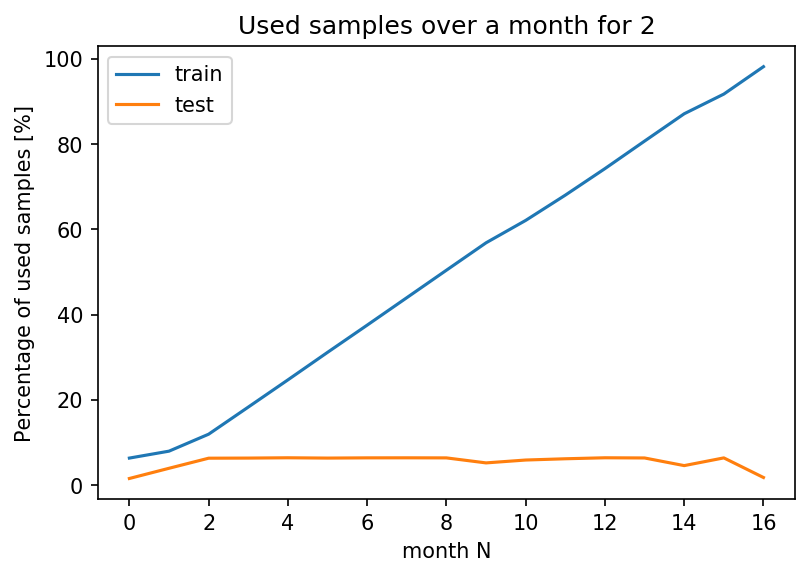
\includegraphics[width=.7\textwidth]{Figures/EC/DYN/tst_tr_b1.png}
	\label{fig:dyn_data_1}
\end{figure}

We can also plot how the amount of data changes for all buildings.
This can be seen on figure \ref{fig:data_used_for_training}.

\begin{figure}[H]
	\centering
	\caption{"Data used for training"}
	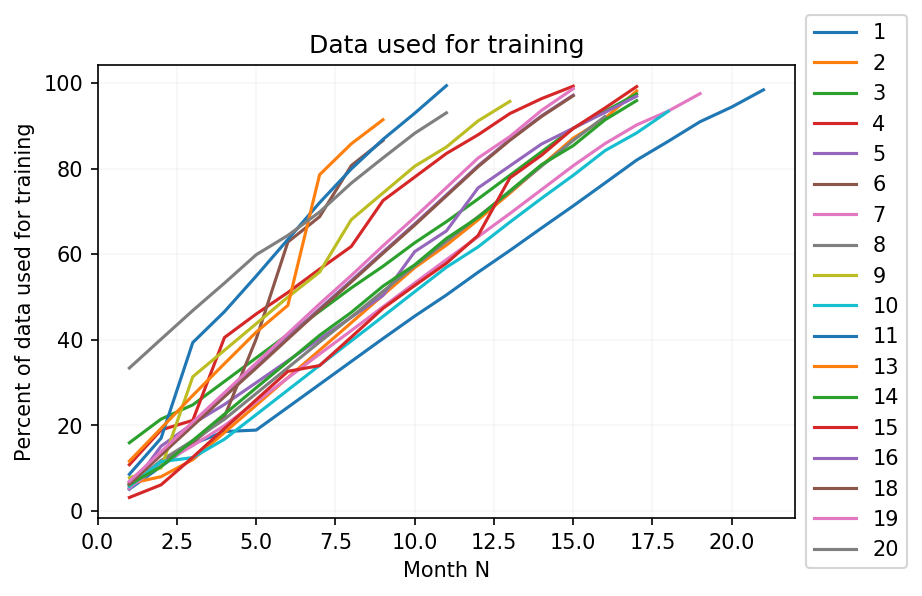
\includegraphics[width=.7\textwidth]{Figures/EC/DYN/data_used_for_training_all.png}
	\label{fig:data_used_for_training}
\end{figure}

To analyze the results, at least 1 year of usable data should be available. 
Figure \ref{fig:data_used_for_training_removed} shows only buildings containing at least one year of data.
\begin{figure}[H]
	\centering
	\caption{"Data used for training, with removed buildings"}
	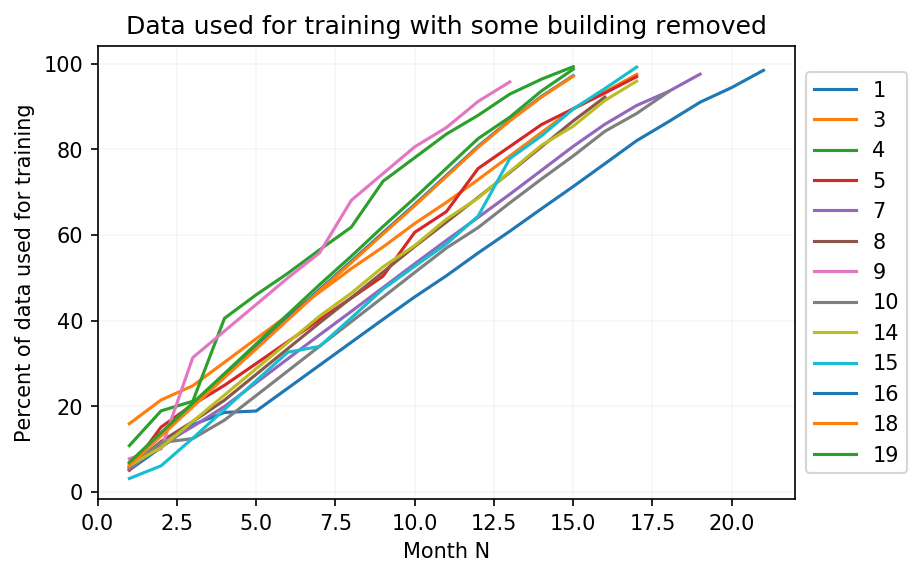
\includegraphics[width=.7\textwidth]{Figures/EC/DYN/data_used_for_training_removed_short.png}
	\label{fig:data_used_for_training_removed}
\end{figure}

Similarly, we can check how test data changes over the months. 
In this case, data is not being aggregated, but only one month of it is used at a time.
Figure \ref{fig:data_used_for_testing} shows, that after one year
the amount of data used for training starts to decline. 
To get more accurate results we will only observe the performance using one year of data. 

\begin{figure}[H]
	\centering
	\caption{"Data used for training, with removed buildings"}
	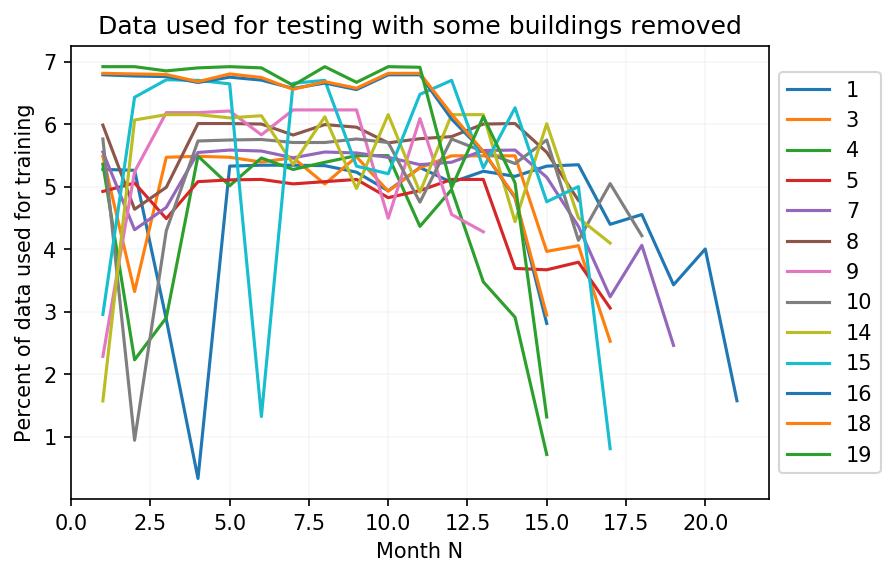
\includegraphics[width=.7\textwidth]{Figures/EC/DYN/data_used_for_testing.png}
	\label{fig:data_used_for_testing}
\end{figure}

\subsection{Results}

To show the effect of training data on the metric, the figure \ref{fig:efect_of_data_on_metric} is presented.
The figure \ref{fig:efect_of_data_on_metric} contains 12 months of 
data for each house, since some have 17 months of data,
they never reach the 100 \% mark.

\begin{figure}[H]
	\centering
	\caption{"Effect of new data on metric"}
	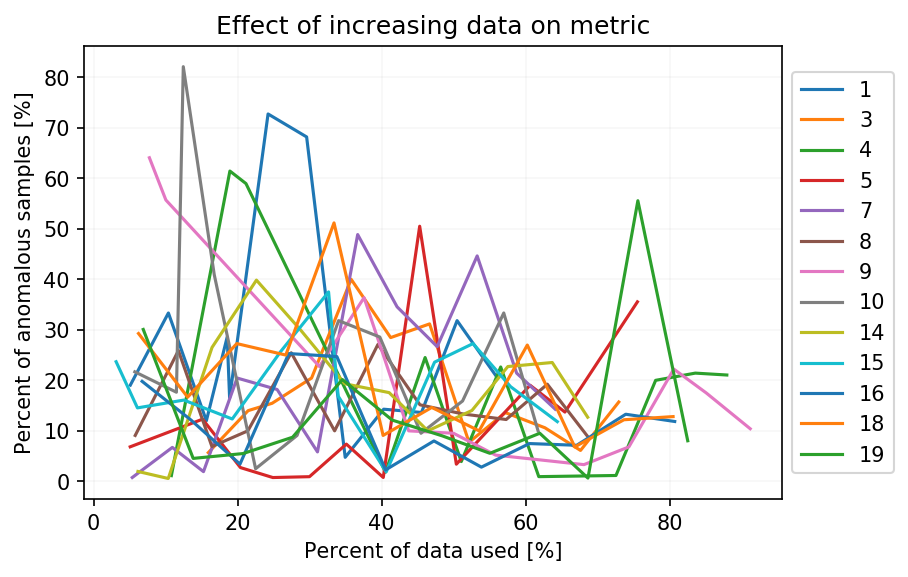
\includegraphics[width=.7\textwidth]{Figures/EC/DYN/efect_of_data_on_metric.png}
	\label{fig:efect_of_data_on_metric}
\end{figure}

Figure \ref{fig:efect_of_data_on_metric} shows, that in most cases, results converge towards 80 \%. 
In some cases, the results are good from the beginning, but sooner or later the routine rate will dip. 
With more data, these dips become smaller and less frequent. 
If the behavior in the household radically changes, it can still lead to a dip.

\begin{figure}[H]
	\centering
	\caption{"Metric over 12 months"}
	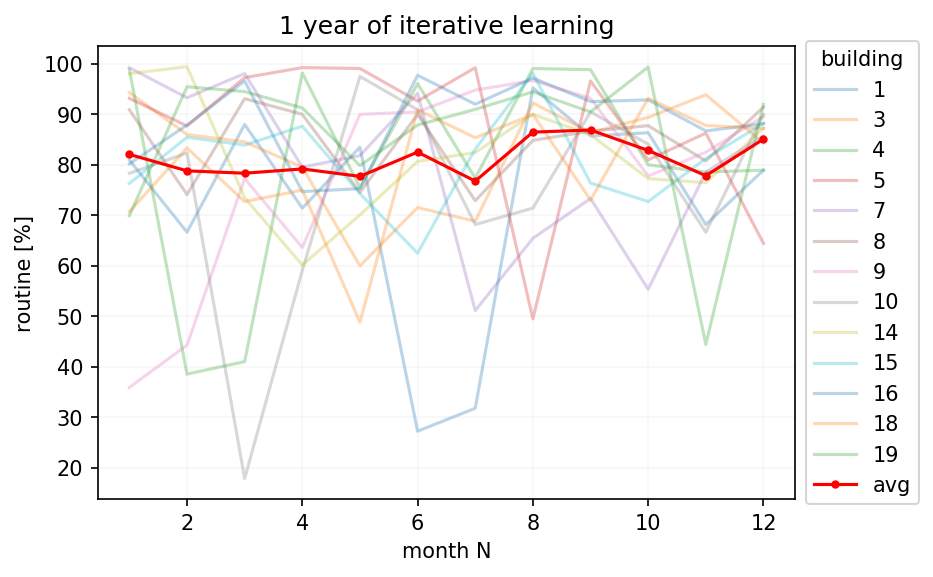
\includegraphics[width=.7\textwidth]{Figures/EC/DYN/1_year_of_iterative_learning_avg.png}
	\label{fig:1_year_of_iterative_learning_avg}
\end{figure}

Figure \ref{fig:1_year_of_iterative_learning_avg} shows how the same data can also be presented so that it shows how the metric changes over a year.
The same as in the previous figure we can observe the dips getting less frequent and smaller. 
Here we can also observe the average line. 
Interestingly enough, due to a large number of buildings, it seems to be sticking at around 80 \%.
Even though the average is oscillating, it is increasing and approaching the 85 \% mark.


\subsection{Discussion}

It is hard to compare these results to the ones from normal learning.
Even though the same data was used, different sections were used.

Let's take the last point on the graph where the average is at 85 \% mark for an example.
Here, the amount of training data is different, since we limited it to one year. 
The train set is also different since only last month was used, and not 20 \%. 
There are many differences in train and test sets, therefore we can not compare them.
The results do prove that the method works and that the true performance is at around the expected 80 \%.

By increasing the amount of data, the algorithm becomes more stable.
In some cases, where users' behavior does not change, the algorithm could work
from the first month forward. In other cases, where behavior is more dynamic, 
the algorithm could need a month or two to stabilize. 

An important thing to keep in mind is that the routine of the users does not increase with more data,
our perceived one does. 

\subsection{Conclusion}

The question that we tried to answer was:
is this method good enough to be able to efficiently detect anomalies? 
The question that should be asked is,
is the behavior of the users periodic enough, to 
be able to efficiently detect the anomaly?
The answer is: yes, it is.


